\chapter{Mean-Variance QTL Mapping on a Background of Variance Heterogeneity}
\label{chap:bvh}

\section{Introduction}



\section{Statistical Methods}

This section reviews four approaches for modeling the effect of a single QTL on the phenotypic mean and/or variance: the standard linear model, Levene's test, Cao's tests, and our preferred procedure based on the DGLM. For each approach we describe a set of alternative procedures for evaluating significance (\ie, calculating p-values) that provide varying degrees of protection against the impact of BVH and distributional assumptions more generally. 
The following section, Data and Simulations, then describes a simulation study that assesses the approaches and p-value procedures, and a dataset to which they are applied genomewide.

\subsection{Definitions}

  We start by defining three partially overlapping classes of QTL:
  \begin{description}
      \item[mQTL:] a locus containing a genetic factor that causes heterogeneity of phenotype mean,
      \item[vQTL:] a locus containing a genetic factor that causes heterogeneity of phenotype variance, and
      \item[mvQTL:] a locus containing a genetic factor that causes heterogeneity of either phenotype mean, variance, or both --- a generalization that includes the other two classes.
  \end{description}
  In addition, since we restrict our attention to QTL mapping methods that test genetic association with a phenotype one locus at a time, we distinguish two sources of variance effects:
  \begin{description}
    \item[Foreground Variance Heterogeneity (FVH):] effects on the variance that arise from the locus under consideration (the focal locus);
    \item[Background Variance Heterogeneity (BVH):] effects on the variance that arise from outside of the focal locus, \eg, from another locus or an experimental covariate.
  \end{description}

  %The remainder of this section reviews a selection of currently used methods for detecting mQTL, vQTL, or mvQTL, namely: the standard linear model, Levene's test, the DGLM, and Cao's test \citep{Cao2014}; this is preceded by a note about our use of several alternative methods for significance evaluation (\ie, calculating p-values) at both a single locus and genomewide. Then we describe a simulation study examining power and false positive rate for each method at single loci. 

\subsection{Procedures to evaluate the significance of a single test}

  In comparing different statistical approaches and their sensitivity to BVH, namely the effect of BVH on power and false positive rate (FPR), it is important to acknowledge that various measures could be taken to make significance testing procedures more robust to model misspecification in general and to BVH specifically.
  The significance testing methods considered here are frequentist, involving the calculation of a test statistic $T$ on the observed data followed by an estimation of statistical significance based on a conception of $T$'s distribution under the null.
  However, BVH constitutes a departure of distributional assumptions, and in any rigorous applied statistical analysis when departures are expected it would be typical to consider protective measures such as, for example, transforming the response to make asymptotic assumptions more reasonable, or the use of computationally intensive procedures, such as those based on bootstrapping or permutation, to evaluate significance empirically. 

  % To allow fair comparisons that bring out the best in each approach, when testing a single hypothesis (\eg, a single locus), as done in the later simulation study, we therefore control the false positive rate using four distinct procedures; when applying the different approaches to a genomewide dataset, as done in our reanalysis study, we integrate these procedures with a procedure to adjust for multiple testing.

  %The power of each method and its robustness to BVH, or distributional assumptions more generally, will depend not only its intrinsic ability to capture on 
  %The power of each method and its robustness to BVH, or distributional assumptions more generally, will depend on the specifics of how that method is applied and its significance evaluated.
  %In particular, all the methods considered here are frequentist, involving the calculation of a test statistic $T$ followed by an estimation of statistical significance based on a conception of $T$'s null distribution. 
  %Yet in any rigorous applied statistical analysis, when it is expected that the data may deviate from assumptions, it is typical to consider the use of protective measures that make a given test more robust. These include, for example, transforming the response to make asymptotic assumptions more reasonable, or the use of computationally intensive procedures, such as those based on bootstrapping or permutation, to evaluate significance empirically.
  %A key feature of the simulations and data analysis is the presence of factors that lie outside the main focus of interest, such as BVH, and their ability to violate null distribution assumptions to disrupt significance testing. Many of the tests considered here assume that the response is distributed normally, after accounting for modeled factors. But in the presence of factors that are not modeled, and that perhaps are not easily modelable, those assumptions are often violated and the corresponding p-values are biased. 
  %The robustness of each method to BVH, or distributional assumptions more generally, will depend on how that method is applied.
  %Yet in any rigorous applied statistical analysis, when deviation from assumptions is expected, it is typical to consider the use of protective measures that make a given test more robust. These include, for example, transforming the response to make asymptotic assumptions more reasonable, or the use of computationally intensive procedures, such as those based on bootstrapping or permutation, to evaluate significance empirically.
  % Since each test considered is frequentist, involving the calculation of a test statistic $T$ followed by a determination of significance under the null, 
  %First, however, we note that since the impact of BVH will depend in part on each method's reliance on parametric assumptions, it would be unfair to compare alternative methods without also considering standard statistical adjustments that would make each one more robust. In particular, when deviation from assumptions is expected, a rigorous applied statistical analysis would typically consider protective measures such as transforming the response, or the use of empirical significance testing based on permutation. 

  Nominal significance (\ie, the p-value for a single hypothesis test) is evaluated using four distinct procedures. The first two rely on asymptotics:
  \begin{enumerate}
      \item Standard: The test statistic $T$ is computed on the observed data and compared with its asymptotic distribution under the null.
      \item Rank-based inverse normal transform (RINT): As for standard, except observed phenotypes $\{y_i\}_{i=1}^n$ are first transformed to strict normality using the function $\text{RINT}(y_i)=\Phi^{-1}[(\text{rank}(y_i) - \sfrac{3}{8})/(n+\sfrac{1}{4})]$, where $\Phi$ is the normal c.d.f. and $\text{rank}(y_i)$ is gives the rank (from $1,\dots,n$) \citep{Beasley2009}.
  \end{enumerate}
  The second two determine significance empirically based on randomization: the test statistic $T$ is recomputed as $T^{(r)}$ under randomizations of the data $r=1,\dots,R$, and the resulting set of statistics $\{T^{(r)}\}_{r=1}^R$ is used as the empirical distribution of $T$ under the randomized null.
  Two alternative randomizations are considered:
  \begin{enumerate}
      \item[3.] Residperm: we generate a pseudo-null response $\{y^{(r)}_i\}_{i=1}^n$ based on permuting the residuals of the fitted null model, \citep{Freedman1983,good2013permutation}, a process recently applied in the field of QTL mapping by \cite{Cao2014}.
      \item[4.] Locusperm: we leave the response intact, instead permuting the rows of the design matrix (or matrices) that differentiate(s) the null from alternative model.
      % This procedure is the single-locus analogue of the permutation approach to genome-wide FWER control proposed by \cite{Churchill1994}, extended where appropriate to accommodate variance effects as described below.
  \end{enumerate}

\subsection{Procedure to evaluate genomewide significance}

  In the context of a genome scan, where many hypotheses are tested, we aim to control the genomewide 
  FPR, namely the family-wise error rate (FWER), the probability of making at least one false positive finding across the whole genome.
  This is done following the general approach of \citet{Churchill1994}, which is closely related to the locusperm procedure described above, and which we refer to as genomeperm.
  Briefly, we perform an initial genome scan, recording test statistics $\{T_l\}_{l=1}^{L}$ for all $L$ loci.
  Then for each randomization $r=1,\dots,R$, and for only the parts of the model that distinguish the null from the alternative model, the genomes are permuted among the individuals; the scan is then repeated to yield simulated null test statistics $\{T^{(r)}_l\}_{l=1}^{L}$ of which the maximum, $T^{(r)}_\text{max}$, is recorded.
  The collection of $\{T^{(r)}_\text{max}\}^R_{r=1}$ from all $R$ such permutations is then used to fit a generalized extreme value distribution (GEV) \citep{Dudbridge2004}, and the quantiles of this are used to estimate FWER-adjusted p-values for each $\{T_l\}_{l=1}^L$.

  % This process is the genomewide analogue of the locusperm procedure described above, so we refer to it as ``genomeperm''.
 
 % the maximum, $T_\text{max}$, recorded. 

  % The methods described above control the false positive rate of a single hypothesis test.
  % In the context of a genome-wide association study, however, each test must be evaluated in the context of the many tests that are conducted. Here control the family-wise error rate (FWER) using the 
  % permutation approach of 
  % \citet{Churchill1994}, whereby the genome scan is repeated many times on pseudo-null datasets generated
  %  by permuting the genomes of the mapping population and the maximum observed statistic from each pseudo-null genome scan is recorded.
  % The threshold to control FWER at $\alpha$ is then estimated by the $1-\alpha$ quantile of the collection of per-scan maxima.
  % To achieve a more precise estimate of the threshold for any given number of permutations, an extreme value density (EVD) can be fitted to the collection of maxima and the $1-\alpha$ quantile of that density can be taken as the threshold \citep{Dudbridge2004}.

  % This approach, that combines permutations and a fitted EVD, has an additional benefit relevant to comparing and co-visualizing tests with different null densities.
  % We map the association statistic at each locus through the cumulative distribution function of the fitted EVD, putting all tests on a comparable scale.
  % The ``$p$ value'' that results from this procedure should be intrepreted as the probability of observing at least one statistic this high or higher over the genome.

\subsection{Standard linear model (SLM) for detecting mQTL}

  The standard model of quantitative trait mapping uses a linear regression based on the approximation of \cite{Haley1992} and \cite{Martinez1992} to interval mapping of \cite{Lander1989a}.
  The effect of a given QTL on quantitative phenotype $y_i$ of individual $i=1,\dots,n$ is modeled as
  % The evidence against the null hypothesis is quantified by comparing the maximum likelihood fit of the null model, in which the locus effects are zero, with that of an alternative model, in which the locus effects are their likelihood-maximizing values.
  % Both the null and the alternative model take the form:
  \begin{align}
    y_i \sim \N(m_i, \sigma^2)
  \end{align}
  where $\sigma^2$ is the residual variance and $m_i$ is a linear predictor for the mean, defined, in what we term the ``full model'', as
  \begin{equation}
    \text{Full model:} \quad  m_i = \mu + \mathbf{x}_i\T\bm{\beta} + \mathbf{q}_i\T\bm{\alpha}\,,
    \label{eq:slm-alt}    
  \end{equation}
  where $\mu$ is the intercept, $\bx_i$ is a vector of covariates with effects $\bm{\beta}$, and $\bq_i$ is a vector encoding the genetic state at the putative mQTL with corresponding mQTL effects $\bm{\alpha}$.
  In the case considered here of biallelic loci arising from a cross of two founders, A and B, the genetic state vector $\bm{q}_i=(a_i,d_i)\T$ is defined as follows: when genotype is known, for genotypes $(\text{AA},\text{AB}, \text{BB})$, the additive dosage is $a_i=(0,1,2)$ and the dominance predictor is $d_i=(0,1,0)$; when genotype is available only as estimated probabilities $p(\text{AA})$, $p(\text{AB})$ and $p(\text{BB})$, following \citep{Haley1992,Martinez1992}, we use the corresponding expectations, $a_i=2p(\text{AA})+p(\text{AB})$ and $d_i=p(\text{AB})$.

  The test statistic for an mQTL is based on comparing the fit of the full model, acting as an alternative model, with that of a null that omits the locus effect, namely,
  \begin{equation}
    \text{Null model:}\quad  m_i = \mu + \mathbf{x}_i\T\bm{\beta} \,.\label{eq:slm-null}
  \end{equation}
  Since the regression in each case provides a maximum likelihood fit, the test statistic used here is likelihood ratio (LR) statistic, $T=2(\ell_1-\ell_0)$, where $\ell_1$ and $\ell_0$ are the log-likelihoods under the alternative and the null respectively. For the biallelic model, the asymptotic test is the likelihood ratio test (LRT) whereby under the null, $T\sim\chi^2_2$. (Note: Alternative evaluation using the F-test is in general more precise but for our purposes provides equivalent results.)

  The residperm approach to empirical significance evaluation of $T$ proceeds as follows.
  We first fit the null model (\autoref{eq:slm-null}) to obtain predicted values $\widehat{m}_i = \bm{x}_i\T\hat{\bbeta}$ and estimated residuals $\widehat{\veps}_i$ such that $y_i = \widehat{m}_i + \widehat{\veps}_i$.
  Then, for each randomization $r=1,\dots,R$, we generate pseudo-null phenotypes $\{y^{(r)}_i\}^n_{i=1}$ as
  \[
    \quad y_i^{(r)} = \widehat{m}_i + \widehat{\veps}_{\pi_r(i)}\,,
  \]
  where if $\bm{\pi}_r$ is a vector containing a random permutation of the indices $i=1,\dots,n$, then $\pi_r(i)$ is its $i$th element, mapping index $i$ to its $r$th permuted version.
  % of the $r$th (randomly drawn) permutation of the indices $1, \dots, n$.
  The null and alternative models are then fitted to $\{y_i^{(r)}\}^n_{i=1}$ to yield $\ell_1^{(r)}$ and $\ell_0^{(r)}$, and hence $T^{(r)}$.

  In the locusperm approach to empirical significance, the response is unchanged but permutations are applied to the locus genotypes. 
  For each randomization $r$, the full model $m_i$ is
  \begin{equation}\label{eq:slm_perm_alt}
    \text{Permuted full model:}\quad m_i = \mu + \mathbf{x}_i\T\bm{\beta} + \mathbf{q}_{\pi_r(i)}\T\bm{\alpha}
  \end{equation}
  where $\pi_r(i)$ is as defined for residperm above.
  This full model fit yields $\ell_1^{(r)}$, and then $T^{(r)} = 2(\ell_1^{(r)} - \ell_0)$.
  Note that $\ell_0^{(r)}$ need not be recomputed after randomization because because only the rows of the design matrices that are unique to the alternative model are permuted and thus $\ell_0^{(r)} = \ell_0$.
  Genomeperm applies locusperm genomewide: specifically, in each randomization $r=1,\dots,R$, the same permutation, $\bm{\pi}_r$, is applied to all $L$ loci.

  % For each permutation $r$ and genetic locus, $l$, the permuted full model is fit to yield $T^*_{r, l}$.
  % For each permutation, the maximum test statistic across all loci is recorded yielding $\{T^*_{\text{max}}\}_{r=1}^{R}$, which is used to estimate the generalized extreme value distribution used to control FWER as described above.
  % }

  % Empirical evaluation is attractive because asymptotic evaluation requires that the null model be true (when evaluating a locus that truly has no effect on the phenotype).
  % In fact, the null model is never exactly true and it is left to scientists to assess the extent to which the disconnect between the null model and the true data-generating process invalidates the asymptotic theory.
  % Additionally, empirical evaluation lends itself naturally to controlling family-wide error rate when the effective number of tests is hard to evaluate \citep{Dudbridge2008}.
  % For these reasons, empirical evaluation of statistical significance is often preferred for QTL mapping \citep{Churchill1994}.

  % Thus, the empirical threshold to control FPR at $\alpha$ is then the $1-\alpha$ quantile of the collected statistics.
  % This threshold is typically estimated by the $1-\alpha$ sample quantile of the collected LRs, but can also be estimated by fitting an extreme value density (EVD) to the collected LRs and calculating its $1-\alpha$ quantile \citep{Stephenson2002,Dudbridge2004}.

\subsection{Levene's Test (LV) for detecting vQTL}
  Levene's test is a procedure for differences in variance between groups that can be used to detect vQTL.
  Suppose individuals are in $G$ mutually exclusive groups $g=1,\dots,G$. Let $g[i]$ denote the group to which individual $i$ belongs, denote $g$th group size as $n_g=\sum_{i=1}^n \indicator{g[i]=g}$, and $g$th group mean as $\bar{y}_g=n_g^{-1}\sum_{i=1}^n y_i \indicator{g[i]=g}$. 
  Then denote the $i$th absolute deviation as $z_i =|y_i-\bar{y}_{g[i]}|$, the group mean of these as $\bar{z}_g=n_g^{-1}\sum_{i=1}^n z_i\indicator{g[i]=g}$ and overall mean $\bar{z} = n^{-1}\sum_{i=1}^n z_i$. Levene's $W$ statistic is then
  \begin{equation}\label{eq:LeveneW}
    W = \frac{
      \sum_{g=1}^G n_g\left( \bar{z}_g - \bar{z}\right)^2
    }{
      (G - 1)
    }
    \left[\frac{\sum_{i=1}^n (z_i - \bar{z}_{g[i]})^2}{(n - G)}\right]^{-1}\,,
  \end{equation}
  which under the null model of no variance effect follows the $F$ distribution as $W \sim F(N - G, G - 1)$ \citep{Levene1960}.
  Note that replacing means of $y$ with medians gives the related Brown-Forsythe test \citep{Brown1973}, and replacing all instances of $z$ with $y$ in \autoref{eq:LeveneW} gives the ANOVA $F$ statistic.

  Levene's test does not lend itself naturally to the residperm approach because it does not explicitly involve a null model to split the data into hat values and residuals.
  We therefore use the null model from the SLM (\autoref{eq:slm-null}) to approximate the residperm procedure with \Lev.
  To execute the locusperm procedure, for each randomization $r$, the group labels are permuted among the individuals, which is equivalent to replacing all instances of $g[i]$ above with $g[\pi_r(i)]$, with $\pi_r(i)$ defined as above.
  A corresponding genomewide procedure, although not performed here, would ensure that each randomization $r$ applies the same permutation $\bm{\pi}_r$ across all loci. 

\subsection{Cao's Tests}

  \cite{Cao2014} elaborates the SLM to have a variance parameter that differs by genotype, \ie,
  \begin{align}
    y_i &\sim \N(m_i, \,\sigma_i^2),
  \end{align}
  where $m_i$ is the linear predictor, $\sigma^2_i$ is the variance of the $i$th individual. These are defined in what we term the ``full model'' as
  \begin{equation}\label{eq:cao_full}
    \text{Full model:}\quad
    \begin{cases}
      \enskip m_i &= \mu + \mathbf{x}_i\T\bm{\beta} + \mathbf{q}_i\T\bm{\alpha}\\
      \enskip \sigma_i^2 &= \phi_{g[i]}
    \end{cases}
    \,,
  \end{equation}
  where $g[i]$ indexes the genotype group to which $i$ belongs, and $\{\phi_g\}^G_{g=1}$ are the variances of the $g=1,\dots,G$ genotype groups. Thus an individual's variance is entirely dictated by its genotype, and that genotype must be categorically known (or otherwise assigned).
  \citet{Cao2014} fits this model using a two-step, profile likelihood method, which in our applications we observe to be indistinguishable from full maximum likelihood (\autoref{fig:cao_profile_accurate}).
   
  \cite{Cao2014} describes tests for mQTL, vQTL and mvQTL based on comparing a full model against three different null models; we detail these tests below in our notation, denoting them respectively \Caom, \Caov, and \Caomv.

  \subsubsection{\Caom test for detection of mQTL}
    The \Caom test involves an LRT between {Cao's full model} and {Cao's no-mQTL model}:
    \begin{equation}\label{eq:caom_null}
      \text{Cao's no-mQTL model:}\quad
      \begin{cases}
        \enskip m_i &= \mu + \mathbf{x}_i\T\bm{\beta}\\
        \enskip \sigma_i^2 &= \phi_{g[i]}
      \end{cases}
      \,,
    \end{equation}
    To execute the residperm procedure for \Caom, pseudo-null phenotypes are generated using $\widehat{m}_i$ and $\widehat{\veps}_i$ from Cao's no-mQTL model (\autoref{eq:caom_null}).
    The locusperm procedure respecifies the full model (\autoref{eq:cao_full}), leaving the variance model unchanged and specifying the mean predictor as $m_i =\mu + \mathbf{x}_i\T\bm{\beta} + \mathbf{q}_{\pi_r(i)}\T\balpha$.
    The genomeperm procedure similarly applies the locusperm procedure genomewide, ensuring each randomization $r$ applies the same permutation $\bm{\pi}_r$ to the mean specification across all loci.

  \subsubsection{\Caov for detection of vQTL}
    The \Caov test involves an LRT between {Cao's full model} and {Cao's no-vQTL model}:
    \begin{equation}\label{eq:caov_null}
      \text{Cao's no-vQTL model:}\quad
      \begin{cases}
        \enskip m_i &= \mu + \mathbf{x}_i\T\bm{\beta} + \mathbf{q}_i\T\bm{\alpha}\\
        \enskip \sigma_i^2 &= \sigma^2
      \end{cases}
      \,,
    \end{equation}
    where the unsubscripted $\sigma^2$ is a single, overall residual variance. This null model is identical to the alternative model in the SLM (\autoref{eq:slm-alt}).

    To execute the residperm procedure for \Caov, pseudo-null phenotypes are generating using $\widehat{m}_i$ and $\widehat{\veps}_i$ from Cao's no-mQTL model (\autoref{eq:caov_null}).
    The locusperm procedure respecifies the full model (\autoref{eq:cao_full}), leaving the mean sub-model unchanged and specifying the variance predictor as $\sigma_i^2 = \phi_{g[\pi(i)]}$.
    The genomeperm procedure applies the locusperm procedure genomewide, ensuring each randomization $r$ applies the same permutation $\bm{\pi}_r$ to the variance specification across all loci.

  \subsubsection{\Caomv for detection of generalized mvQTL}
    The \Caomv test involves an LRT between {Cao's full model} and {Cao's no-QTL model}:
    \begin{equation}\label{eq:caomv_null}
    \text{Cao's no-QTL model:}\quad
    \begin{cases}
      \enskip m_i &= \mu + \mathbf{x}_i\T\bm{\beta}\\
      \enskip \sigma_i^2 &= \sigma^2
    \end{cases}
    \,.
    \end{equation}
    This null model is identical to the null model in the SLM (\autoref{eq:slm-null}).

    To execute the residperm procedure for \Caomv, pseudo-null phenotypes are generated using $\widehat{m}_i$ and $\widehat{\veps}_i$ from Cao's no-QTL model (\autoref{eq:caomv_null}).
    The locusperm procedure specifies the mean predictor as $m_i = \mu + \mathbf{x}_i\T\bm{\beta} + \mathbf{q}_{\pi(i)}$ and the variance predictor as $\sigma_{g[i]}^2 = \phi_{[\pi(i)]}$.
    The genomeperm procedure applies the locusperm procedure genomewide, ensuring each randomization $r$ applies the same permutation $\bm{\pi}_r$ to the mean and variance specifications across all loci.


\subsection{Double Generalized Linear Model (DGLM)}

  The DGLM models the phenotype $y_i$ via two linear predictors as
  \[
    y_i \sim \N(m_i, \,\sigma_i^2)\,,\\
    \quad\text{where}\quad\sigma^2_i = \sigma^2 \times \exp(v_i)\,
  \]
  where $m_i$ predicts the phenotype mean and $v_i$ predicts the extent to which the baseline residual variance $\sigma^2$ is increased in individual $i$.
  In what we term the ``DGLM full model'', these are specified as

  \begin{equation}\label{eq:dglm_full}
    \text{Full model:}\quad
    \begin{cases}
    \enskip m_i &= \mu + \mathbf{x}_i\T\bm{\beta} + \mathbf{q}_i\T\bm{\alpha}\\
    \enskip v_i &= \mathbf{z}_i\T\bm{\gamma} + \mathbf{q}_i\T\bm{\theta}
    \end{cases}
    \,,
  \end{equation}
  where $\mu$ is the intercept, $\mathbf{z}_i$ is a vector of covariates (which may be identical to $\mathbf{x}_i$),
  $\bm{\gamma}$ is a vector of covariate effects on $v_i$,
  and $\bm{\theta}$ is a vector of locus effects on $v_i$.

  As with Cao's full model, the DGLM full model can be compared, in a likelihood ratio test, with various null models to test for mQTL, vQTL \citep{Ronnegard2011a}, or mvQTL.
  A full maximum likelihood fitting procedure for the DGLM was provided by \cite{Smyth1989}.
  
  \subsubsection{DGLM\textsubscript{M} for detecting mQTL:}
    For detecting mQTL, we use an LRT of the {DGLM full model} in \autoref{eq:dglm_full} against the {no-mQTL model}:
    \begin{equation}\label{eq:dglmm_null}
      \text{No-mQTL model:}\quad
      \begin{cases}
      \enskip m_i &= \mu + \bx_i\T\bm{\beta}\\
      \enskip v_i &= \bz_i\T\bm{\gamma} + \mathbf{q}_i\T\bm{\theta}
      \end{cases}
      \;,
    \end{equation}
    where the LR statistic has asymptotic distribution $T\sim\chi^2_2$.

    To execute the residperm procedure for \DGLMm, pseudo-null phenotypes are generated using $\widehat{m}_i$ and $\widehat{\veps}_i$ from the Equation \ref{eq:dglmm_null}.
    The locusperm procedure respecifies the mean predictor as $m_i = \mu + \mathbf{x}_i\T\bm{\beta} + \mathbf{q}_{\pi(i)}\T\bm{\alpha}$ and does not modify the variance predictor.
    The genomeperm procedure similarly applies the locusperm procedure genomewide, ensuring each randomization $r$ applies the same permutation $\bm{\pi}_r$ to the mean specification across all loci.

  \subsubsection{DGLM\textsubscript{V} for detecting vQTL:}
    For detecting vQTL, we use an LRT of the {DGLM full model} in \autoref{eq:dglm_full} against the {no-vQTL model}:
    \begin{equation}\label{eq:dglmv_null}
      \text{No-vQTL model:}\quad
      \begin{cases}
      \enskip m_i &= \mu + \mathbf{x}_i\T\bm{\beta} + \mathbf{q}_i\T\bm{\alpha}\\
      \enskip v_i &= \mathbf{z}_i\T\bm{\gamma}
      \end{cases}
      \,,
    \end{equation}
    where the LR statistic has asymptotic distribution $T\sim\chi^2_2$.

    To execute the residperm procedure for \DGLMv, pseudo-null phenotypes are generated using $\widehat{m}_i$ and $\widehat{\veps}_i$ from the Equation \ref{eq:dglmv_null}.
    The locusperm procedure does not modify the variance predictor and respecifies the mean predictor as $v_i = \mathbf{z}_i\T\bm{\gamma} + \mathbf{q}_{\pi(i)}\T\bm{\theta}$.
    The genomeperm procedure similarly applies the locusperm procedure genomewide, ensuring each randomization $r$ applies the same permutation $\bm{\pi}_r$ to the variance specification across all loci.

  \subsubsection{DGLM\textsubscript{MV} for detecting mvQTL:}
    For detecting mvQTL, we use an LRT of the {DGLM full model} in \autoref{eq:dglm_full} against the {no-QTL model}:
    \begin{equation}\label{eq:dglmmv_null}
      \text{No-QTL model:}\quad
      \begin{cases}
      \enskip m_i &= \mu + \mathbf{x}_i\T\bm{\beta} \\
      \enskip v_i &= \mathbf{z}_i\T\bm{\gamma}
      \end{cases}
      \,,
    \end{equation}
    where the LR statistic has asymptotic distribution $T\sim\chi^2_4$.

    To execute the residperm procedure for \DGLMmv, pseudo-null phenotypes are generated using $\widehat{m}_i$ and $\widehat{\veps}_i$ from the Equation \ref{eq:dglmmv_null}.
    The locusperm procedure respecifies the mean predictor as $m_i = \mu + \mathbf{x}_i\T\bm{\beta} + \mathbf{q}_{\pi(i)}\T\bm{\alpha}$ and the variance predictor as $v_i = \mathbf{z}_i\T\bm{\gamma} + \mathbf{q}_{\pi(i)}\T\bm{\theta}$.
    The genomeperm procedure similarly applies the locusperm procedure genomewide, ensuring each randomization $r$ applies the same permutation $\bm{\pi}_r$ to the mean and variance specifications across all loci.


% \subsection{Genomewide significance}

% \subsection{Assessing genomewide significance}

% [ROUGH THOUGHTS]

% Under genomewide permutation:
% \begin{itemize}
% \item SLM: standard and locusperm are identical. With no mean covariates, residperm is also identical. RINT is effectively identical.
% \item Levene: standard and locusperm are identical. RINT effectively so.
% \item DGLM: standard and locusperm are identical only for DGLMmv?
% \end{itemize}


% standard: perm
% residperm: at each perm, do whole genome
% locusperm: permute q together.

\section{Data and Simulations}

Simulation was used to assess the ability of the eight tests described above to distinguish each of the three types of QTL --- pure mQTL, pure vQTL, and mixed mvQTL --- from a null locus in the presence and absence of background variance heterogeneity (BVH).
% The role of each of the eight tests 
Tests are distinguished by their ability to accommodate and target foreground variance heterogeneity (FVH) and background variance heterogeneity (Table~\ref{tab:tests}).
% In scenarios with BVH, the tests that can make use of the covariate that drives the BVH (the DGLM-based tests) were tested both with and without knowledge of that covariate.

\begin{table}
    % \renewcommand{\familydefault}{\sfdefault}\normalfont
    \centering
    \begin{tabular}{l|l|p{7cm}}
    \hline
     \textbf{Category} & \textbf{Test} & \textbf{Description} \\
    \hline
    mQTL        & SLM       & Conventional test of mean differences;\newline allows neither FVH nor BVH \\
    mQTL        & \Caom{}   & Allows FVH, but not BVH \\
    mQTL        & \DGLMm{}  & Allows FVH and BVH \\
    \hline
    vQTL        & \Lev{}    & Conventional test of variance differences;\newline detects FVH, does not allow BVH \\
    vQTL        & \Caov{}   & Detects FVH, does not allow BVH \\
    vQTL        & \DGLMv{}  & Detects FVH, allows BVH \\
    \hline
    mvQTL       & \Caomv{}  & Detects FVH, does not allow BVH \\
    mvQTL       & \DGLMmv{} & Detects FVH and allows BVH \\
    \hline
    \end{tabular}
    \caption[
      The eight tests that were evaluated in the simulation studies.
    ]
    {
      The eight tests that were evaluated in the simulation studies. FVH: foreground variance heterogeneity. BVH: background variance heterogeneity.
    }
    \label{tab:tests}
\end{table}

In each simulation, $n = 300$ observations were simulated as
\[
    y_i \sim \N(q_i\T \alpha, \exp(\mathbf{z}_i\T\bm{\gamma} + q_i\T \theta))
\]
where $y_i$ is the phenotype of individual $i$,
    ${q_i}$ is the genotype,
    and $\mathbf{z}_i$ is the indicator vector for the factor that drives BVH in scenarios where it is present.
    In each simulation, each row of $\mathbf{q}$ (each ${q}_i$) is drawn randomly from [-1, 0, 1] with probability (0.25, 0.5, 0.25) mimicking an F2 intercross.
    Across all simulations, $\bm{Z}$ is fixed to be an indicator matrix mapping the first 60 observations to group 1, the next 60 to group 2, ... and the last 60 to group 5.

% \[
%     \bm{y} \sim \text{N}(\bm{q}\alpha, \exp(\bm{Z\gamma} + \bm{q}\theta))
% \]
% where $\bm{y}$ is the phenotype,
%     $\bm{q}$ is the genotype,
%     and $\bm{Z}$ is the design matrix associated with the factor that drives BVH in scenarios where it is present.
%     In each simulation, each element of $\bm{q}$ is drawn randomly from [-1, 0, 1] with probability (0.25, 0.5, 0.25) mimicking an F2 intercross.
%     Across all simulations, $\bm{Z}$ is fixed to be an indicator matrix mapping the first 60 observations to group 1, the next 60 to group 2, ... and the last 60 to group 5.
Values of $\alpha$, $\theta$, and $\bm{\gamma}$ differentiate the eight simulation scenarios as described below.

\subsection{Scenarios}

Simulations varied in two dimensions: locus effect (four options) and BVH (two options) for a total of eight simulation scenarios.
Each of the eight scenarios was examined in $S = 10,000$ simulation trials.
Locus effect sizes were chosen such that all QTL were detectable with approximately 70\% power at a 5\% false positive rate for traditional tests in the absence of BVH.
Comprehensive details on the simulation setup are described in \textbf{Supplementary Materials}.

The four options for a simulated locus effect were as follows:
\begin{enumerate}
    \item null locus: The locus has no effect on phenotype.
    \item pure mQTL: The locus has an additive effect on the phenotype mean that explains $5\%$ of the total variance.
    \item pure vQTL: The locus has an additive effect on the log standard deviation that is detectable with approximately 70\% power at a 5\% false positive rate for traditional tests in the absence of BVH. %scale that is approximately equally detectable by \Lev in the absence of BVH as an mQTL that explains 5\% of phenotype variance is by the SLM.
    \item mixed mvQTL: The locus has both an additive mean effect that explains $3.25\%$ of phenotype variance and an additive variance effect that is approximately equally detectable.
\end{enumerate}
% \subsubsection*{Locus effect (more detailed version):}
% \begin{enumerate}
%     \item null locus: The locus has no effect on phenotype.
%     \item pure mQTL: The locus explains $5\%$ of phenotype variance, implying genotype-wise means of $[-0.23, 0, 0.23]$ in the no BVH scenario and $[-0.25, 0, 0.25]$ in the BVH scenario.
%     \item pure vQTL: The locus has an additive effect of $0.17$ on the log standard deviation, implying genotype-wise standard deviations of $[0.844, 1, 1.185]$ in the no BVH scenario and 15 distinct standard deviations in the BVH scenario.
%     \item mixed mvQTL: The locus has a mean effect that explains $3.25\%$ of phenotype variance and variance effect of $0.136$ on the log standard deviation, implying genotype-wise means of [-0.18, 0, 0.18] and standard deviations of $[0.873, 1, 1.145]$ in the no BVH scenario and means of $[-0.20, 0, 0.20]$ and 15 distinct standard deviations in the BVH scenario.
% \end{enumerate}
The two options for simulated BVH were as follows:
\begin{enumerate}
    \item absent: Nothing, except for possibly the locus (if a vQTL or mvQTL), influences the residual variance.  ($\bm{\gamma} = [0, 0, 0, 0, 0]$)
    \item present: $\bm{\gamma} = [-0.4, -0.2, 0, 0.2, 0.4]$, resulting in group-wise standard deviations in the null locus and mQTL scenarios of approximately $[0.67, 0.82, 1, 1.22, 1.49]$.
    In the vQTL and mvQTL scenarios, these BVH effects combine additively with the locus effects on the log standard deviation scale, yielding 15 distinct standard deviations.
    These effect sizes generate a spectrum of standard deviations across groups that are consistent with those observed in the real data reanalysis that follows.
\end{enumerate}


\subsection{Tests and Significance}
In each scenario, eleven tests were applied, and four procedures were used to assess the statistical significance of each test, for a total of 32 test-procedures.

The eleven tests comprise four tests for detecting mQTL: \LM, \Caom, and \DGLMm  with and without modeling the variance covariate; four for detecting vQTL: \Lev, \Caov, \DGLMv with and without modeling the variance covariate; and three for detecting mvQTL: \Caomv and \DGLMmv with and without modeling the variance covariate, as described in \textbf{Methods}.

The eleven tests, however, contain some redundancy, and so in the main text we report results from only eight. Specifically, for a given type of QTL, the DGLM model that omits variance covariates is equivalent to the corresponding Cao's test, and, barring computational errors in fitting, should give equivalent results (as was observed); results from these DGLM models are therefore omitted from the main text, but for completeness are reported in the supplement.

The four procedures for evaluating the statistical significance were: standard, RINT, residperm, and locusperm, as described in the \textbf{Methods}.
% For standard and RINT versions, the theoretical null distributions were $\chi^2_1$ for \LM, \Caom, \DGLMm, \Caov, and \DGLMv, $\chi^2_2$ for \Caomv and \DGLMmv, and $F_{1,299}$ for \Lev.

\subsection{Evaluation of tests and procedures}

Tests and procedures for assessing statistical significance were evaluated based on their receiver operating characteristics (ROC) and their ability to accurately control the FPR to the nominal level. 
ROC curves display the ability of a test to discriminate between two conditions by plotting FPR against power for all possible cutoffs.

In this case, the ROC curve reflects the ability of a test to discriminate between QTL and null loci.
%, by plotting FPR against power for all p-value cutoffs.
%at a given cutoff $c\in[0,1]$, the discriminatory ability of a set of simulated p-values denote the number of true positives, false positives and false negatives as $\text{TP}_c$, $\text{TN}_c$ and $\text{FP}_c$,
%then $\text{TPR}_c=\text{TP}_c/(\text{FN}_c+\text{TP}_c)$ and
%$\text{FPR}_c=\text{FP}_c/(\text{FP}_c+\text{TP}_c)$.
%and the TPR, the fraction of non-null (QTL) true positive fraction for all cutoffs $c$.
Specifically, for a given method and cutoff $c$, the FPR was the fraction null simulations in which the nominal p-value $p$ was less than $c$; the power is the fraction of times this happened in non-null (\ie, QTL) simulations.
%For example, when $c=0$ the false positive fraction and true positive fraction are both 0, because no simulations returned a $p$ value less than 0.
%And when $c=1$, the false positive fraction and true positive fraction are both 1, because all simulations returned a $p$ value less than 1.
A test was said to accurately control FPR when, for all $c$, $\text{FPR} = c$; it was said to ``dominate'' another test when it had higher power across all FPRs.

The ROC curve cannot immediately distinguish between tests that accurately control FPR and those that do not.
We added a symbol to each ROC curve at the point where $c = 0.05$.
%, which we term the ``ROC point''. % minimize new terminology
In cases where the point falls on the vertical line at FPR = 0.05, it reflects accurate FPR control.
In cases where the point falls to the left or right of the vertical line it reflects a conservative or anti-conservative test, respectively.
QQ plots, provided in the supplementary material provide a more holistic view on the FPR control of each test and procedure.

\subsection{Leamy \etal Summary of Original Study}

\citet{Leamy2000} backcrossed mice from strain CAST/Ei, a small, lean strain, into mouse strain M16i, a large, obese strain.
Nine F1 males were bred with 54 M16i females to produce a total of 421 offspring (208 female, 213 male), which were genotyped at 92 microsatellite markers across the 19 autosomes and phenotyped for body composition and morphometric traits.
We retrieved all available data on this cross, which included marker genotypes, covariates, and eight phenotypes (body weight at five ages, liver weight, subcutaneous fat pad thickness, and gonadal fat pad thickness), from the Mouse Phenome Database \citep{Grubb2014a}, and estimated genotype probabilities at 2cM intervals across the genome using the hidden Markov model in \texttt{R/qtl} \citep{Broman2003}.

This mapping population has been studied for association with several phenotypes:
    asymmetry of mandible geometry \citep{Leamy2000},
    limb bone length \citep{Leamy2002,Wolf2006},
    organ weight \citep{Leamy2002,Wolf2006,Yi2006},
    fat pad thickness \citep{Yi2005,Yi2006,Yi2007},
    and body weight \citep{Yi2006}.
The most relevant prior study to this reanalysis, \cite{Yi2006}, used standard methods to identify QTL for body weight at three weeks on chromosomes 1 and 18. However, we were not able to reproduce this result, despite following their analysis as described.

% Of the many phenotypes measured, eight were available on the Mouse Phenome Database \citep{Grubb2014a} --- body weight at five ages, liver weight, subcutaneous fat pad thickness, and gonadal fat pad thickness. 
% All eight phenotypes exhibited BVH due to father, and we performed both traditional QTL mapping using the SLM and mean-variance QTL mapping using the DGLM on all eight phenotypes.
% For body weight at three, six, and nine weeks of age, one, three, and one new QTL were identified, respectively.
% For the other five traits, no new QTL were identified.
% For brevity, we describe in detail only the new QTL for body weight at three weeks of age.
% \RC{Scripts to conduct all these analyses and their results are included in supplementary file X.}{necessary?  If not, delete.}


\subsection{Availability of Data and Software}

Analyses were conducted in the \texttt{R} statistical programming language \citep{RCoreTeam2017}.
The simulation studies used the implementation of the standard linear model from package \texttt{stats}, \Lev from \texttt{car}, Cao's tests as published in \cite{Cao2014} and the DGLM tests in package \texttt{dglm}.
The reanalyzed dataset is available on the Mouse Phenome Database \citep{Grubb2014a} with persistent identifier \mpdidentifier.

The entire project, including data and all analysis scripts, is available as a Zenodo repository at \zenodourl.
There are six files stored in this repository.
Files S1, S2, and S3 contain the R scripts necessary to replicate the simulation studies and their analysis, relying on the \texttt{plotROC} package to make ROC plots \citep{sachs2017plotroc}.
File S4 contains the data from \cite{Leamy2000} that was reanalyzed.
File S5 contains the attempted replication of the original analysis \citep{Yi2006} and file S6 contains the new analysis, using package \texttt{vqtl}.



% \WV{
% \texttt{R} package \texttt{vqtl} implements mean-variance QTL mapping, including the permutation procedure for significance testing and plotting functions for interpretation and dissemination of results.
%     It is interoperable with the popular \texttt{R/qtl} package, so reseachers can easily extend their mapping study to try this analysis.
%     A thorough illustration of its typical use was published as a companion [companionA].
%     It is freely available on CRAN.
%     Development history, new features, and bug reporting are available at \texttt{github.com/rcorty/vqtl}.
% }{Your previous text. 1) You need to include where you got the Leamy data here, along with all significant packages used, and whatever scripts are needed to redo the simulations. 2) Check for compliance with G3 requirements; you could also have Dan and Paul look over it since they've just had to do this themselves. Below I include for reference the stuff from Paul's paper.}

\section{Results}

\subsection{Simulation study on single locus testing}

\begin{figure}
  \centering
  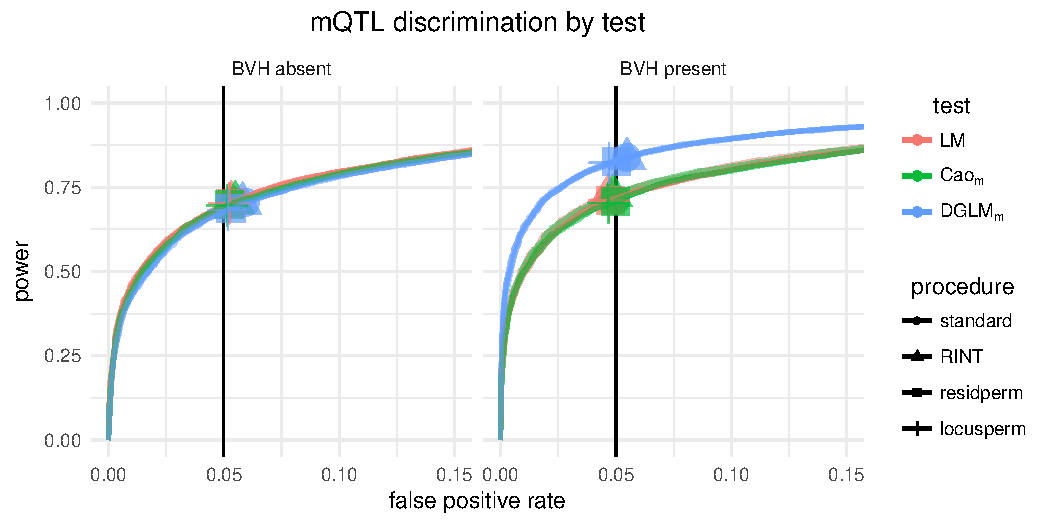
\includegraphics[width = \linewidth]{images/simple_rocs_mqtl_all_facet_by_bvh.pdf}
  \caption[
    ROC curves for detection of mQTL in presence and absence of BVH.
  ]
  {
    ROC curves for detection of mQTL in presence and absence of BVH.
    Lines are drawn for three different mQTL tests in \autoref{tab:tests} and four significance procedures, with a point (circle, square, triangle, tick) corresponding to nominal significance at $p=0.05$ (more details in \textbf{Data and Simulations}).
    \DGLMm dominates \Caom and SLM in the presence of BVH, accurately controlling FPR with the locusperm and residperm procedures, but not the standard and RINT procedures, which have FPR of 0.058 and 0.060 (\autoref{tab:05}).
  }
  \label{fig:roc_mqtl}
\end{figure}

Simulations were performed to examine the ability of the eight tests listed in \autoref{tab:tests} to detect nonzero effects belonging to their target QTL types (mQTL, vQTL, mvQTL), and to control the number of false positives when no such QTL effects were present. This was done both in the presence and absence of background variance heterogeneity, and for each test, with p-values calculated by each of the four alternative p-value generation procedures (standard, RINT, residperm, locusperm). The full combination of settings is listed in \autoref{tab:05}, which also lists results pertaining to a nominal FPR of 0.05, and described in more detail in \textbf{Data and Simulations}.

\subsubsection{All three mQTL tests have equivalent performance in the absence of BVH.}

All three mQTL tests --- the standard linear model, the \Caom test and \DGLMm --- accurately controlled FPR under all four significance testing procedures (\autoref{fig:roc_mqtl}, left panel, \autoref{fig:mqtl_tests_null_qqs}, left column, and \autoref{tab:05}, column 1, top third).
And all twelve test-procedure combinations had indistinguishable power to detect mQTL, in the range [0.692, 0.706] (\autoref{tab:05}, column 2 and \autoref{fig:mqtl_rocs_supp}).

These simulation results do not favor any one test over another, but they do favor the standard and RINT assessment procedures over the residperm and locusperm in the sense that the latter two yield no additional improvement in FPR control or power for their additional computational cost.
%In the context of a genome scan, however, a permutation-based approach is likely still necessary to control FWER.

\subsubsection{\DGLMm dominates other mQTL tests in the presence of BVH.}

The SLM and \Caom accurately controlled FPR under all four procedures to assess statistical significance (\autoref{fig:roc_mqtl}, right panel, \autoref{fig:mqtl_tests_null_qqs}, right column, and \autoref{tab:05}, column 5, top third).
In contrast, \DGLMm exhibited modest FPR inflation under the standard and RINT procedures, controlling FPR to the nominal level only under the empirical procedures.
Nonetheless, despite requiring an empirical procedure to control FPR, in its power to detect an mQTL under BVH, \DGLMm dominated the other two tests, with power in the range of [0.813, 0.816] compared with the power of SLM and \Caom in the range of [0.689, 0.718] (\autoref{fig:roc_mqtl}, right panel, \autoref{tab:05}).

Based on the results of these simulations, \DGLMm is the preferable mQTL test in the presence of BVH.
But, to accurately control FPR, \DGLMm requires an empirical procedure be used to assess statistical significance; both the residperm and locusperm procedures are capable.


%\RC{The additional power of \DGLMm over the other tests derives from its reweighting of the observations in proportion to their estimated residual variance.}{remove?}


        % The additional power of \DGLMm in the presence of BVH does not come at the cost of increased false positive rate.
        % In both the presence and absence of BVH, all mQTL tests accurately control FPR (\autoref{fig:roc_mqtl} and \ref{fig:null_qqs}).
        % At a nominal FPR of 0.05, they control FPR to the range [0.048, 0.052] (\autoref{tab:05}, column 1, rows 1-12).

        % Based on these results, there is no reason to prefer one mQTL test over another in the absence of BVH.
        % But, in the presence of BVH driven by a known factor, \DGLMm is the preferable mQTL test due to its increased power.

\begin{figure}
  \centering
  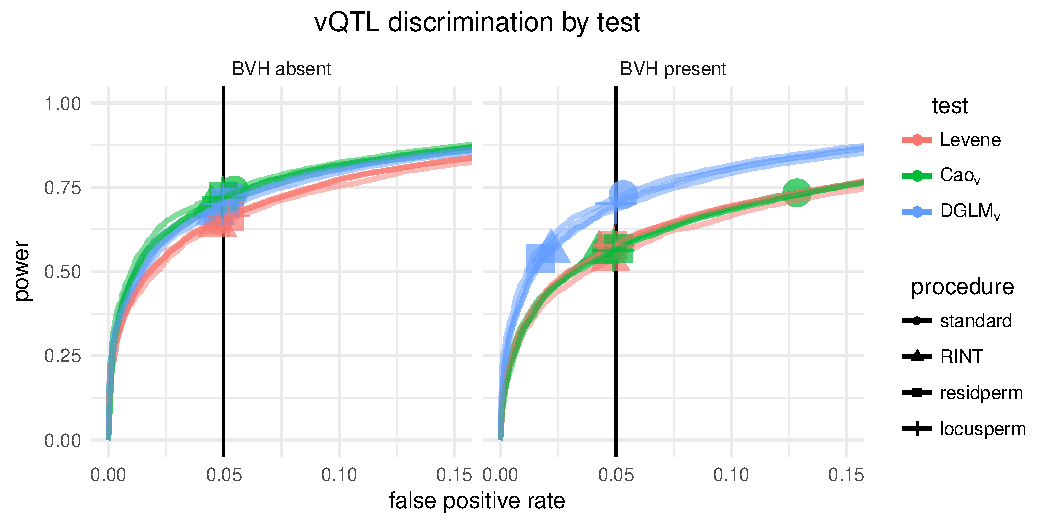
\includegraphics[width = \linewidth]{images/simple_rocs_vqtl_all_facet_by_bvh.pdf}
  \caption[
    ROC curves for detection of vQTL in presence and absence of BVH. 
  ]
  {
    ROC curves for detection of vQTL in presence and absence of BVH. 
    Lines are drawn for three different vQTL tests in \autoref{tab:tests} and four significance procedures, with a point (circle, square, triangle, tick) corresponding to nominal significance at $p=0.05$ (more details in \textbf{Data and Simulations}).
    \DGLMv dominates \Caov and \Lev in the presence of BVH and accurately controls FPR under the standard and locusperm procedures (\autoref{tab:05}).
    \Caov suffers a drastic increase in false positives in the presence of BVH under the standard procedure, and \DGLMv would do the same if there were some unmodeled BVH driver, thus \DGLMv under the locusperm procedure is the preferable test.
    % In the absence of BVH, \DGLMv are \Caov identically powerful and are both more powerful than \Lev (ROC curves with circles are higher in panel 2 and 3 than in panel 1).
    % In the presence of BVH of uknown source all three vQTL tests have nearly identical ability to distinguish vQTL from null loci (all ROC curves with triangles overlap).
    % In the presence of BVH from a known source, \DGLMv recovers most of the power that is lost to BVH of unknown source (in panel 3, ROC curves with squares nearly overlap ROC curves with circles).
    % The only version guaranteed to accurately control FPR is locusperm (all purple shapes are on FPR = 0.05, not true for any other color).
    % See Fig~\ref{fig:vqtl_rocs_supp} for additional views of these results.
  }
  \label{fig:roc_vqtl}
\end{figure}

\subsubsection{Parametric tests dominate Levene's test for vQTL in the absence of BVH.}

In null simulations, \Caov and \DGLMv exhibited slightly anti-conservative behavior using the standard (\ie, asymptotic) significance testing procedure (FPR = 0.053), modestly conservative behavior under the RINT procedure (FPR = 0.043) and slightly conservative behavior under the residperm and locusperm procedures (FPR in the range [0.046, 0.048], \autoref{fig:roc_vqtl}, left panel, \autoref{fig:vqtl_tests_null_qqs}, left column, and \autoref{tab:05}, column 2, middle third).
\Lev, in contrast, was overly conservative using the standard and RINT procedures, but accurately controlled FPR under the empirical procedures (\autoref{fig:vqtl_rocs_supp}).

Despite the variation in FPR control among the test-procedure combinations, \Caov and \DGLMv had more power than \Lev under all procedures (0.724 vs. 0.667).
Thus, the empirical procedures of \Caov and \DGLMv are the preferred vQTL tests in the absence of BVH, because they have the highest power of the test-procedure combinations that are not anti-conservative.
The additional power of \Caov and \DGLMv relative to \Lev is consistent with the fact that they make strong parametric assumptions that are exactly true in these simulations and \Lev does not.

\subsubsection{\DGLMv dominates other vQTL tests in the presence of BVH.}

In the presence of BVH, there were three test-procedure combinations with major departures from accurate FPR control.
\Caov under the standard procedure was drastically anti-conservative, and \DGLMv under both the RINT and residperm procedures was drastically conservative (\autoref{fig:roc_vqtl}, right panel and \autoref{fig:vqtl_rocs_supp}, and \autoref{fig:vqtl_tests_null_qqs}, right column).
\DGLMv dominated \Lev and \Caov, so the standard and locusperm procedure, which accurately control its FPR, seem to be equally preferable and preferable over all other test-procedures.

% \DGLMv under the locusperm procedure has power of 0.713, significantly greater than 0.583, the power of \Lev under the locusperm procedure, the most powerful other test that does not have inflated FPR.
Nonetheless, there is an important caveat that makes locusperm the strongly preferable significance procedure.
In this simulation, there are no BVH driving factors unknown to \DGLMv.
If there were such a factor, \DGLMv under the standard procedure would have the same drastic FPR inflation that \Caov showed under the standard procedure in these simulations (\autoref{fig:vqtl_rocs_supp}~(a), third panel).
In contrast, the presence of a unknown or unmodeled BVH driving factor does not inflate the FPR of \DGLMv under the locusperm procedure.
Due to the practical difficulty of excluding the possibility of an unknown BVH driver, the most reliable way to guard against covert FPR inflation without giving up the additional power of \DGLMv is to use the locusperm procedure.

        % The FPR and TPR of the RINT and residperm versions of \DGLMv at a nominal FPR of 0.05 are  of [0.021, 0.570] and [0.015, 0.542] respectively (\autoref{tab:05}, columns 5 and 7, middle third).
        % Thus, it appears initially that both the standard and locusperm versions of \DGLMv are equally preferable vQTL tests in the presence of BVH, as both accurately control FPR and have more power than any other test.

        % Upon further inspection, however, there is an important distinction between the standard and locusperm versions of \DGLMv.
        % The standard version of \Caov has a drastically inflated FPR of 0.123 (\autoref{tab:05}, column 4, middle third), while the locusperm version maintains accurate FPR control.
        % \Caov and \DGLMv differ only in whether the BVH driver is modeled.
        % If there were some unknown or unmeasured BVH driver that \DGLMv were unable to account for, it would have the same properties as \Caov in this simulation.
        % Thus, \textbf{unless the possibility of an unknown BVH-driver can be excluded, locusperm is the unique amongst significance testing procedures studied here in accurately controlling the FPR of \DGLMv in the presence of BVH} (\autoref{fig:vqtl_rocs_supp} (c)).

        % of uknown source all test-versions have nearly identical ROC, but all are dominated by the tests conducted in the absence of BVH.
        % With two exceptions, all test-versions accurately control FPR as well.
        % The exceptions are the standard version of \Caov and \DGLMv, which have drastically inflated FPR (Figs.~\ref{fig:roc_vqtl}, \ref{fig:vqtl_rocs_supp}, and \ref{fig:vqtl_tests_null_qqs}).
        % In the presence of BVH from a known source, \DGLMv recovers the discrimination ability that was lost with the introduction of BVH and therefore  dominates all other tests conducted in the presence of BVH.
        % In this setting, \DGLMv's standard and locusperm verions accurately control FPR, while the other versions do not (Figs.~\ref{fig:roc_vqtl}, \ref{fig:vqtl_rocs_supp}, and \ref{fig:vqtl_tests_null_qqs}).

        % Based on these results, the RINT versions of \Caov and \DGLMv are the preferable vQTL test when BVH is known to be absent and when its source is uknown.
        % The residperm and locusperm versions of these tests have the same power and FPR but are slower to compute.
        % In the presence of BVH of known source, the locusperm version of \DGLMv is the preferable test.
        % Though its standard version has the same power and FPR control when there are strictly no unknown BVH drivers, it leaves the researcher exposed to the danger of a covertly inflated FPR if there is some unknown BVH driver.

    \begin{figure}
        \centering
        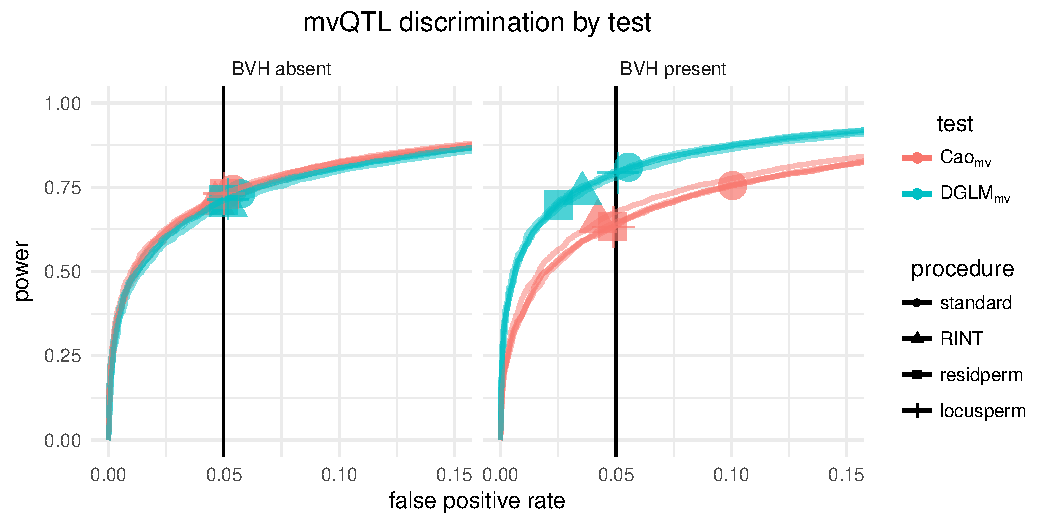
\includegraphics[width = \linewidth]{images/simple_rocs_mvqtl_all_facet_by_bvh.pdf}
        \caption[
          ROC curves for detection of mvQTL in presence and absence of BVH. 
        ]
        {
            ROC curves for detection of mvQTL in presence and absence of BVH. 
            Lines are drawn for two different mvQTL tests in \autoref{tab:tests} and four significance procedures, with a point (circle, square, triangle, tick) corresponding to nominal significance at $p=0.05$ (more details in \textbf{Data and Simulations}).
            mvQTL tests combined the responses of mQTL tests and vQTL tests to BVH, yielding a situation in which \DGLMmv dominates \Caomv, but only accurately controls FPR under the locusperm procedure (\autoref{tab:05}).
            The anti-conservative nature of the standard procedure follows from the patterns observed in mQTL tests and the conservative nature of the RINT and residperm procedures follows from the patterns observed in vQTL tests.
            % In the absence of BVH and in the presence of BVH from an unknown source, \Caomv and \DGLMmv have identical ability to distinguish mvQTL from null  loci.
            % In the presence of BVH from a known source, \DGLMmv dominates \Caomv.
            % See Fig~\ref{fig:mvqtl_rocs_supp} for additional views of the ROC plots.
        }
        \label{fig:roc_mvqtl}
    \end{figure}

    \subsubsection{mvQTL mirrors vQTL testing; \DGLMmv dominates \Caomv in the presence of BVH.}
        As with vQTL tests, there was little to distinguish any test or procedure in the absence of BVH except for the modest conservative nature of the RINT procedure and the concomitant decrease in power (\autoref{fig:roc_mvqtl}, left panel and \autoref{tab:05}, columns 1 and 4, bottom third).
        
        In the presence of BVH, however, \DGLMmv dominates \Caomv, with the standard and locusperm procedures accurately controlling FPR (\autoref{fig:roc_mvqtl}, right panel and \autoref{fig:mvqtl_tests_null_qqs}, right column).
        As with vQTL testing, due to the difficulty in ruling out BVH from an unknown source and the inflated FPR that results from such BVH under the standard procedure, the \DGLMmv under the locusperm procedure is the recommended test for mvQTL.


\subsubsection{In the presence of BVH, the rank-based inverse normal transformation fails to correct anti-conservative behavior of \DGLMm and over corrects that of \DGLMv and \DGLMmv}
A consistent feature of the simulations involving detection of variance effects, whether vQTL or mvQTL, is that FPR control and power is affected, for better or worse, by applying the RINT to the response.

In the presence of BVH, \DGLMm under the standard procedure was anti-conservative (FPR = 0.058 at $\alpha = 0.05$).
The RINT procedure had no efficacy in returning this test to accurate FPR control (FPR = 0.060).

In the case of vQTL detection in the presence of BVH, \Caov under the standard procedure had a drastically inflated FPR (0.123) and the RINT procedure over-corrected it (FPR = 0.044).
Similarly, the RINT procedure disrupted \DGLMv, which accurately controlled FPR under the standard procedure, causing overly conservative behavior (FPR = 0.021).

As always, in the presence of BVH, the mvQTL tests exhibited a mixture of the patterns observed in mQTL tests and vQTL tests.
Both \Caomv and \DGLMmv were anti-conservative under the standard procedure, illustrating their relations to \Caov and \DGLMm respectively.
And in both cases, the RINT procedure drove an over-correction into the realm of over conservatism (FPR = 0.046 and 0.038 respectively).

In summary, the RINT procedure is unhelpful in the context of the \DGLMm: it inflates the FPR of a test that is appropriately sized under standard procedures.
But, in the context of vQTL testing with BVH from an unknown source, it has one useful and important property:
    pre-processing the phenotype with the RINT, leads to vQTL tests that are conservative rather than anti-conservative, decreasing the probability of false positives at the expense of false negatives.

% are erratic enough in their FPR control that the locusperm procedure is preferable, even before considering its utility in FWER control.}{Surely this underplays RINT's advantages? Soften. Locusperm will not always be possible to implement, and so if RINT is better than nothing we should say so.}

% The RINT procedure introduced a modest FPR inflation into the \DGLMm test
% 

% Under BHV, standard and RINT is anti-conservative for \DGLMm. RINT lowers the anti-conservative standard (although too much so) for \Caov, \Caomv; RINT over-lowers the accurate standard for \DGLMv and the slightly inflated \DGLMmv.

% Absent BVH, RINT is slightly conservative for detecting vQTL with \Caov and \DGLMv.


        % \Caomv and \DGLMmv exhibited a combination of the patterns observed with mQTL tests and vQTL tests (\autoref{fig:roc_mvqtl}, \autoref{fig:mvqtl_rocs_supp}, and \autoref{fig:mvqtl_tests_null_qqs}).

        % \paragraph{In the absence of BVH,} the standard version of \Caomv and \DGLMmv accurately controlled FPR at 0.05 (\autoref{tab:05}) and had identical power at 0.741.
        % The other versions of \Caomv and \DGLMmv were either conservative (RINT and residperm) or more computationally intensive (residperm and locusperm).
        % Thus, in the absence of BVH, the standard version of \Caomv and \DGLMmv are equally preferable and are both more preferable than any other test-version.

        % \paragraph{In the presence of BVH,} however, the mvQTL tests exhibited a similar pattern to the vQTL tests.
        % Specifically, 
        % The same effects of BVH on the testing properties was observed in relation to mvQTL testing that was observed in relation to vQTL testing.
        % Specifically, \DGLMmv dominates \Caomv and only the locusperm version can be relied upon to accurately control FPR in consideration of the possibility of an additional unknown factor driving BVH.

        % The disturbance in FPR control 
        % The introduction of BVH weakens \Caomv and \DGLMmv, as with all vQTL tests, and knowledge of the source of the BVH allows \DGLMmv to recover the lost power (as with \DGLMv) and exceed the power it had in the absence of BVH (as with \DGLMm).

    \begin{table*}
        \centering
        \begin{tabular}{lll llll llll lll}
            \cmidrule[1pt]{1-10}
             &  & \multicolumn{4}{c}{BVH absent} & \multicolumn{4}{c}{BVH present}\\
             \cmidrule(lr){3-6} \cmidrule(lr){7-10} 
             test & version & null & mQTL & vQTL & mvQTL & null & mQTL & vQTL & mvQTL\\
             \cmidrule[1pt]{1-10}
            \LM & standard & 0.050 & 0.706 & 0.056 & 0.510 & 0.051 & 0.701 & 0.050 & 0.508 \\ 
             & RINT & 0.050 & 0.704 & 0.052 & 0.495 & 0.052 & 0.718 & 0.049 & 0.518 \\ 
             & residperm & 0.048 & 0.700 & 0.054 & 0.502 & 0.049 & 0.694 & 0.050 & 0.504 \\ 
             & locusperm & 0.049 & 0.702 & 0.054 & 0.499 & 0.049 & 0.695 & 0.049 & 0.503 \\ 
            \cmidrule[0.1pt]{1-10}
            \Caom & standard & 0.052 & 0.705 & 0.051 & 0.515 & 0.050 & 0.700 & 0.048 & 0.516 \\ 
             & RINT & 0.051 & 0.705 & 0.051 & 0.503 & 0.052 & 0.716 & 0.047 & 0.523 \\ 
             & residperm & 0.049 & 0.697 & 0.049 & 0.503 & 0.048 & 0.695 & 0.047 & 0.508 \\ 
             & locusperm & 0.048 & 0.691 & 0.048 & 0.500 & 0.048 & 0.689 & 0.044 & 0.503 \\ 
            \cmidrule[0.1pt]{1-10}
            \DGLMm & standard & 0.052 & 0.705 & 0.051 & 0.515 & 0.058 & 0.832 & 0.054 & 0.649 \\ 
             & RINT & 0.051 & 0.705 & 0.051 & 0.503 & 0.060 & 0.830 & 0.054 & 0.644 \\ 
             & residperm & 0.049 & 0.696 & 0.049 & 0.504 & 0.052 & 0.816 & 0.046 & 0.629 \\ 
             & locusperm & 0.048 & 0.692 & 0.048 & 0.500 & 0.050 & 0.813 & 0.046 & 0.624 \\ 
            \cmidrule[1pt]{1-10}
            \Lev & standard & 0.045 & 0.049 & 0.660 & 0.462 & 0.046 & 0.046 & 0.577 & 0.393 \\ 
             & RINT & 0.045 & 0.043 & 0.645 & 0.422 & 0.047 & 0.043 & 0.546 & 0.344 \\ 
             & residperm & 0.049 & 0.052 & 0.667 & 0.474 & 0.048 & 0.050 & 0.585 & 0.401 \\ 
             & locusperm & 0.049 & 0.052 & 0.667 & 0.474 & 0.048 & 0.050 & 0.583 & 0.400 \\ 
            \cmidrule[0.1pt]{1-10}
            \Caov & standard & 0.053 & 0.053 & 0.750 & 0.543 & 0.123 & 0.127 & 0.744 & 0.563 \\ 
             & RINT & 0.043 & 0.042 & 0.700 & 0.467 & 0.044 & 0.048 & 0.563 & 0.364 \\ 
             & residperm & 0.047 & 0.051 & 0.729 & 0.519 & 0.045 & 0.054 & 0.572 & 0.388 \\ 
             & locusperm & 0.046 & 0.049 & 0.726 & 0.517 & 0.047 & 0.051 & 0.567 & 0.382 \\ 
            \cmidrule[0.1pt]{1-10}
            \DGLMv & standard & 0.053 & 0.053 & 0.750 & 0.543 & 0.049 & 0.056 & 0.732 & 0.524 \\ 
             & RINT & 0.043 & 0.042 & 0.700 & 0.467 & 0.021 & 0.027 & 0.570 & 0.340 \\ 
             & residperm & 0.048 & 0.051 & 0.729 & 0.520 & 0.015 & 0.018 & 0.542 & 0.329 \\ 
             & locusperm & 0.046 & 0.049 & 0.724 & 0.515 & 0.046 & 0.050 & 0.713 & 0.498 \\ 
            \cmidrule[1pt]{1-10}
            \Caomv & standard & 0.050 & 0.597 & 0.643 & 0.741 & 0.100 & 0.642 & 0.649 & 0.751 \\ 
             & RINT & 0.043 & 0.585 & 0.574 & 0.701 & 0.046 & 0.600 & 0.436 & 0.646 \\ 
             & residperm & 0.046 & 0.587 & 0.618 & 0.728 & 0.050 & 0.514 & 0.507 & 0.632 \\ 
             & locusperm & 0.048 & 0.589 & 0.617 & 0.727 & 0.050 & 0.516 & 0.506 & 0.630 \\ 
            \cmidrule[0.1pt]{1-10}
            \DGLMmv & standard & 0.050 & 0.597 & 0.643 & 0.741 & 0.057 & 0.741 & 0.633 & 0.807 \\ 
             & RINT & 0.043 & 0.585 & 0.574 & 0.701 & 0.038 & 0.715 & 0.445 & 0.726 \\ 
             & residperm & 0.046 & 0.590 & 0.618 & 0.729 & 0.024 & 0.621 & 0.469 & 0.687 \\ 
             & locusperm & 0.046 & 0.590 & 0.617 & 0.728 & 0.051 & 0.723 & 0.601 & 0.788 \\
             \cmidrule[1pt]{1-10}
        \end{tabular}
        \caption[
          Positive rates of mQTL, vQTL, and mvQTL tests.
        ]
        {
            Positive rates of all tests in all scenarios based on 10,000 simulations, 1,000 permutations each to estimate empirical null distributions (residperm and locusperm), and a nominal false positive rate (FPR) of $\alpha = 0.05$.
            Entries in column 1 and 5 through all rows, columns 3 and 7 in the top third, and columns 2 and 6 in the middle third represent FPR.
            The entries in the rest of the table represent power.
            The largest standard error for an FPR is 0.001.
            The largest standard error for a power is 0.0025.
        }
        \label{tab:05}
    \end{table*}


\subsection{Genomewide reanalysis of bodyweight in Leamy et al. backcross}

\begin{figure}
  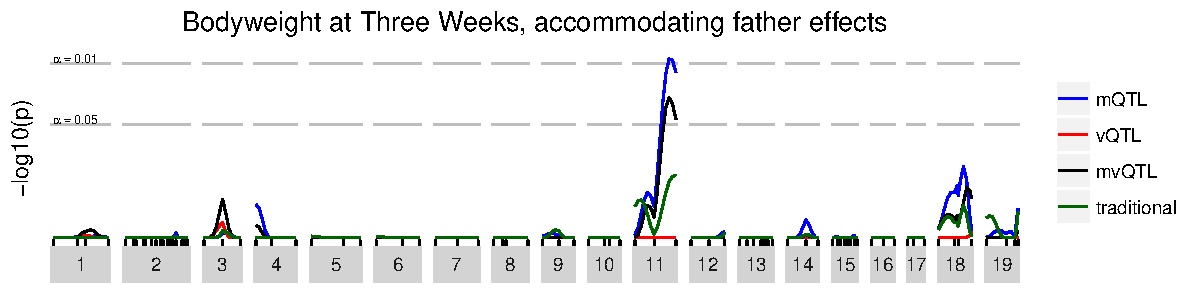
\includegraphics[width = \linewidth]{bw3wk_scan_father_only.pdf}
  \caption[
    FWER-controlling association statistic at each genomic locus for body weight at three weeks.
  ]
  {
    FWER-controlling association statistic at each genomic locus for body weight at three weeks.
    The linear model (green, ``traditional'') does not detect any statistically-significant associations.
    The mQTL test takes into account the heterogeneity of both mean and variance due to which F1 male fathered each mouse in the mapping population and detects one mQTL on chromosome 11.
  }
  \label{fig:genome_scan_dglm}
\end{figure}

To understand the impact of BVH on mean and variance QTL mapping in real data, we applied both traditional QTL mapping, using SLM, and mean-variance QTL mapping, using Cao's tests and the DGLM, to body weight at three weeks in the mouse backcross dataset of \citet{Leamy2000}.
%In both types of analysis, sex and father were included as covariates, and the significance of associations was judged based on 1000 genome permutations.

\subsubsection{Analysis with Traditional QTL Mapping Identifies no QTL.}

We first used a traditional, linear modeling-based QTL analysis, with  sex and father as additive covariates and genomewide significance based on 1000 genome permutations \citep{Churchill1994}.
Although sex was found not to be a statistically significant predictor of body weight ($p = 0.093$ by the likelihood ratio test with 1 degree of freedom), it was included in the mapping model because, based on the known importance of sex in determining body weight, any QTL that could only be identified in the absence of modeling sex effects would be highly questionable.
Father was found to be a significant predictor of body weight in the baseline fitting of the SLM ($p = 9.6 \times 10^{-5}$ by the likelihood ratio test with 8 degrees of freedom) and therefore was included in the mapping model.
% For each permuted scan, the maximum likelihood ratio was recorded and an extreme value density was fitted to the collection of per-permutaion maxima.
% Likelihood ratios observed on the non-permuted data were adjusted to control family-wise error rate by mapping them through the cumulative distribution function of the fitted extreme value density \citep{Dudbridge2004}[CompanionB].

No associations rose above the threshold that controls family-wise error rate to 5\% (\autoref{fig:genome_scan_dglm}, green line).
One region on the distal part of chromosome 11 could be considered ``suggestive'' with FWER-adjusted $p \approx 0.17$.

To test the sensitivity of the results to the inclusion/exclusion of covariates, the analysis was repeated without sex as a covariate, without father as a covariate, and with no covariates.
No QTL were identified in any of these sensitivity analyses.

\subsubsection{Analysis with Cao's tests Identifies no QTL}
The same phenotype was analyzed with Cao's tests, again including sex and father as mean covariates, and using the genome permutation procedures described in \textbf{Methods} were used to control FWER.
No statistically significant mQTL, vQTL, nor mvQTL were identified (\autoref{fig:bw3wk_cao_scan}).

\subsubsection{Analysis with DGLM-based tests Identifies an mQTL}
The same phenotype was analyzed with the DGLM-based tests.
% As with the traditional analysis and the analysis with Cao's tests, sex and father were included as covariates on the mean.
% Additionally, they were included as covariates on the variance.
In a baseline fitting of the DGLM, sex was found not to be a statistically significant predictor of mean or residual variance (mean effect $p = 0.18$, variance effect $p = 0.22$, and joint $p = 0.19$ by the LRT with 1, 1, and 2 d.f.).
But father was found to be a statistically significant predictor of both mean and variance (mean effect $p = 2.0 \times 10^{-7}$, variance effect $p = 1.8 \times 10^{-11}$ , and $p = 4.8 \times 10^{-14}$ by the LRT with 8, 8, and 16 d.f.).
Therefore, following the same reasoning as in the mean model described above, both sex and father were included in the mapping model as covariates of both the mean and the variance.
As with the other tests, the genome permutation procedures described in \textbf{Methods} were used to control FWER.

A genomewide significant mQTL was identified on chromosome 11 (\autoref{fig:genome_scan_dglm}, blue line).
The peak was at 69.6 cM with FWER-adjusted $p=0.011$, with the closest marker being D11MIT11 at 75.7 cM with FWER-adjusted $p=0.016$.
Nonparametric bootstrap resampling, using 1,000 resamples (after \citealt{Visscher1996}), established a 90\% confidence interval for the QTL from 50 to 75 cM.
This region overlaps with the ``suggestive'' region identified in the traditional analysis.

By the traditional definition of percent variance explained, following from a fitting of the standard linear model, this QTL explains 2.1\% of phenotype variance.
Though, given the variance heterogeneity inherent in the DGLM that was used to detect this QTL, this quantity is better considered the ``average'' percent variance explained.
The ratio of the QTL variance to the sum of QTL variance, covariate variance, and residual variance ranges from 1\% to 6\% across the population, based on the heterogeneity of residual variance.

    % \begin{figure}
    %     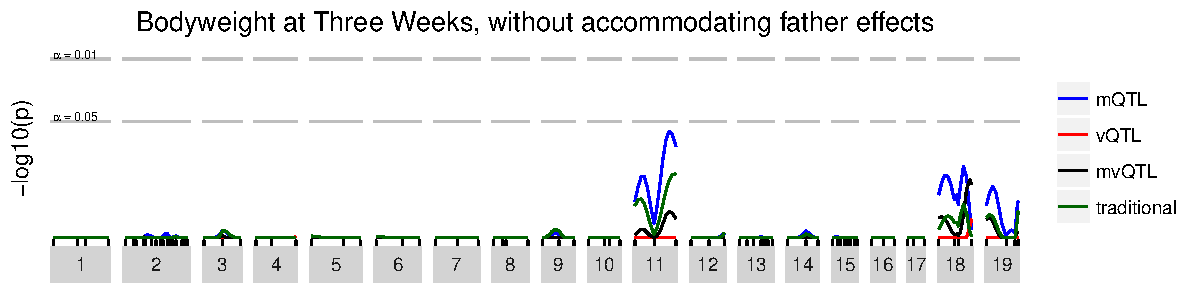
\includegraphics[width = \textwidth]{bw3wk_scan_cao}
    %     \caption{FWER-controlling association statistic at each genomic locus for the ``body weight at three weeks'' phenotype.
    %     The linear model (green, ``traditional'') does not detect any statistically-significant associations.
    %     The mQTL test takes into account the heterogeneity of both mean and variance due to which F1 male fathered each mouse in the mapping population and detects one mQTL on chromosome 11.}
    %     \label{fig:genome_scan_cao_tests}
    % \end{figure}

    \begin{figure}
        \centering
        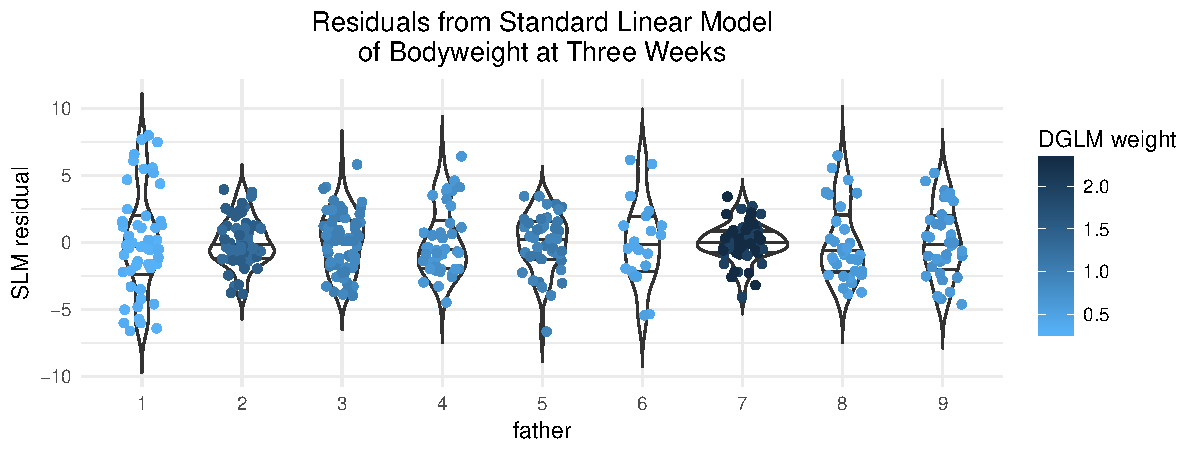
\includegraphics[width = \linewidth]{bw3wk_residuals_by_father.pdf}
        \caption[
          Residuals from the standard linear model for body weight at three weeks, with sex and father as covariates, stratified by father.
        ]
        {
          Residuals from the standard linear model for body weight at three weeks, with sex and father as covariates, stratified by father.
          It is evident that fathers differed in the residual variance of the offspring they produced.
          For example, the residual variance of offspring from father 1 is greater than that of father 2 and 7.
          Here, points are colored by their predicted residual variance in the fitted DGLM with sex and father as mean and variance covariates.
        }
        \label{fig:bw3wk_resids}
    \end{figure}

    \begin{figure}
        \centering
        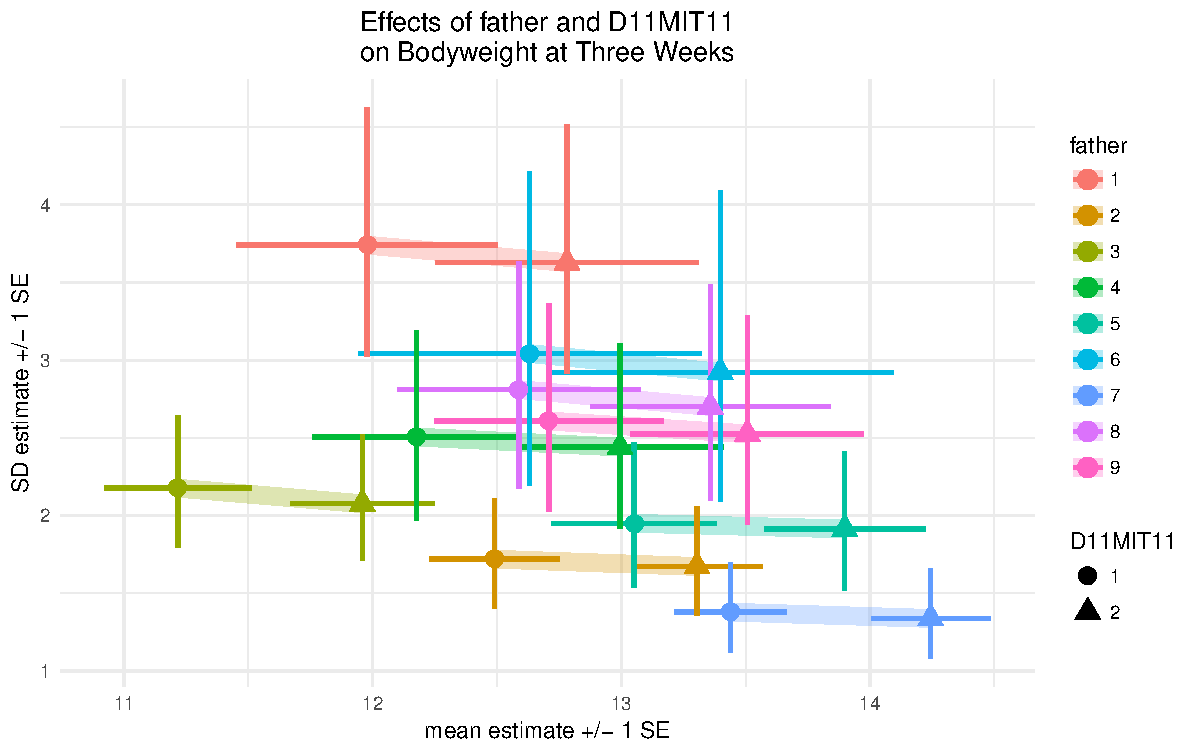
\includegraphics[width = \linewidth]{bw3wk_mean_var_plot_father_D11MIT11.pdf}
        \caption[
          The predictive mean and standard deviation of mice in the mapping population based on father and genotype at the top marker, D11MIT11 on chromosome 11.
        ]
        {
          The predictive mean and standard deviation of mice in the mapping population based on father and genotype at the top marker, D11MIT11 on chromosome 11.
          The genotype effect, illustrated by the colored ribbons is almost entirely horizontal, indicating a difference in means across genotype groups but no difference in variance, consistent with the identification of this QTL as a pure mQTL.
          The father effects, illustrated by the spread of colored crossbars, have both mean and variance components.
          For example, father 7 (blue) has the highest predictive mean and lowest predictive standard deviation.
          His offspring were upweighted in the QTL analysis based on their low standard deviation.
          Father 1 (red) has an average predictive mean and the highest predictive standard deviation.
          His offspring were downweighted in the QTL analysis based on their high standard deviation.
          Note: the effect of sex on phenotype mean and variance was modeled, then marginalized out for readability.
        }
        \label{fig:bw3wk_meanvar}
    \end{figure}

    \subsubsection{Understanding the Novel QTL}

    The mQTL on chromosome 11 was identified by the \DGLMm test, but not by by the standard linear model or Cao's mQTL test.
    The additional power of the \DGLMm test over these other tests relates to its accommodation of background variance heterogeneity (BVH).
    
    Specifically, the DGLM reweighted each observation based on its residual variance, according to the sex and F1 father of the mouse.
    This BVH is visually apparent when the residuals from the standard linear model are plotted, separated out by father (\autoref{fig:bw3wk_resids}).

    % Although sex was found not to be a statistically significant predictor of phenotype mean (p = 0.18) or residual variance (p = 0.21), it was included in both the mean and variance sub-models.
    % The mQTL reported here was not sensitive to the inclusion/exclusion of sex as a mean or variance covariate in the mapping model.

    Some fathers, for example fathers 2 and 7, appear to have offspring with less residual variance than average, whereas others, for example father 1, seem to have offspring with more residual variance than average.
    The DGLM captured these patterns of variance heterogeneity, and estimated the effect of each father on the log standard deviation of the observations (\autoref{fig:bw3wk_meanvar}).
    Based on these estimated variance effects, observations were upweighted (e.g. fathers 2 and 7) and downweighted (e.g. father 1).
    This weighting gave the DGLM-based mapping approach more power to reject the null as compared to the SLM.

    % Could not replicate, so commented out
    % \subsubsection{SLM Reanalysis based on DGLM Insight}
    %     In light of the observed high variance of the offspring of father 1, we removed these mice from the dataset and re-ran the traditional QTL analysis.
    %     The QTL on chromosome 11 was identified as statistically significant.
    %     This finding indicates that the major contribution of the DGLM-based mapping approach in this instance was downweighting the less reliable observations, those from father 1.
    %     Said another way, the highly-variable offspring of father 1 falsely inflated the estimate of the residual variance of all the other mice, which falsely deflated the signal-to-noise ratio and caused the observed difference in means across genotypes to be considered consistent with chance in the SLM.

    % In short, by upweighting mice from less-variable fathers provide more information about the mean of their genotype group than mice from other fathers do.

    % \begin{figure}
    %     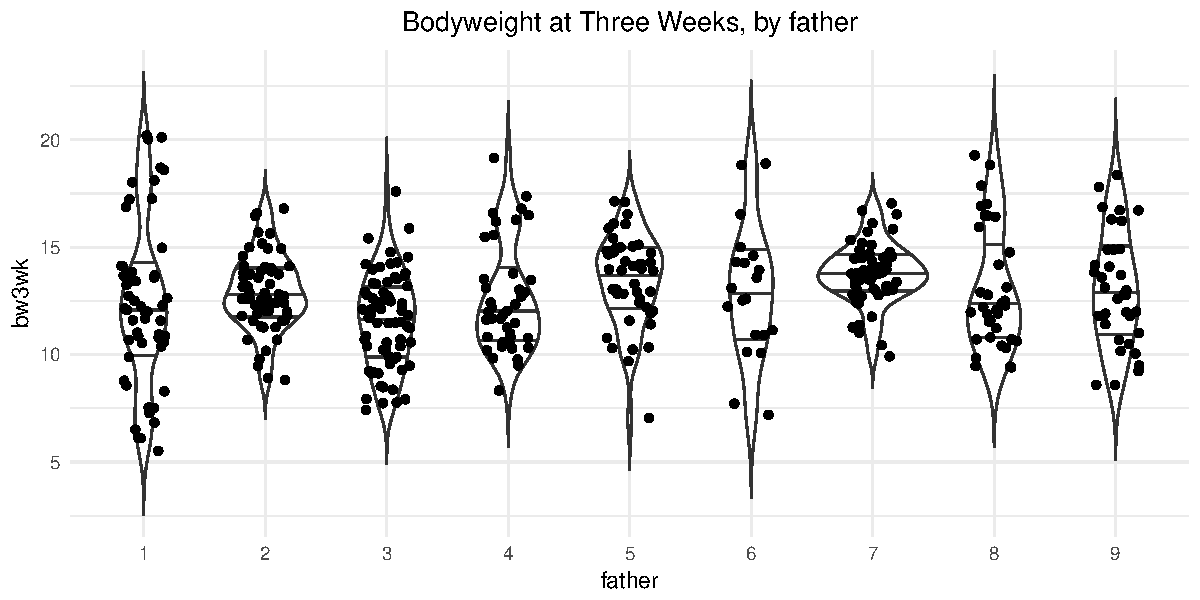
\includegraphics[width = \textwidth]{bw3wk_by_father.pdf}
    %     \caption{body weight at three weeks, stratified by father.
    %     It is evident that fathers differed in the variance of the offspring they produced.
    %     But, 
    %     For example, the residual variance of offspring from father 1 is greather than that of father 2.}
    % \end{figure}

    \subsubsection{Other Phenotypes}
    For brevity, we described in detail only the results of the DGLM-based analysis of body weight at three weeks; but, of the eight phenotypes from this cross available on the Mouse Phenome Database, the mean-variance approach to QTL mapping discovered new QTL in four.
    Five of the eight phenotypes --- body weight at twelve days, three weeks, and six weeks, as well as subcutaneous and gonadal fat pad thickness --- exhibited BVH due to father, and for each we performed both traditional QTL mapping using the SLM and mean-variance QTL mapping using the DGLM.
    For body weight at three weeks and six weeks, we identified one new mQTL and two new vQTL respectively.
    For subcutaneous fat pad thickness, we ``undiscovered'' one mean QTL.
    That is, after reweighting the observations based on the observed variance of each father, two QTL that were detected by the SLM no longer met criteria for statistical significance, as shown in supplementary figures.
    
    %For brevity, we describe in detail only the new QTL for body weight at three weeks of age.
    %\RC{Scripts to conduct all these analyses and their results are included in supplementary file X.}{necessary?  If not, delete.}

\section{Discussion}

The simulation studies revealed that in the presence of background variance heterogeneity (BVH), the DGLM-based tests are uniquely powerful in the detection of mQTL, vQTL, and mvQTL.

Our reanalysis of the Leamy et al. dataset demonstrated that the additional power of \DGLMm in the face of BVH can be used to detect an mQTL that was overlooked by all competitor methods.

\subsection{Detecting and Modeling BVH}
To select the right test and procedure to assess significance, it is important to establish whether there is any BVH present.
We advocate fitting the DGLM with all potential BVH drivers as variance covariates, then including any that are statistically significant as variance covariates in the mapping model to improve power to detect QTL.

% But this approach depends on knowledge of the suspected BVH driver.
% If this factor is unknown or unmeasured, it can still influence the properties of QTL tests, for example inflating the FPR of \Caov and \DGLMv under the standard version.
% One can compare a QQ plot of the data (or residuals from the SLM) against the normal distribution with QQ plots against various $t$ distributions.
% If the tails of the data are better explained by the $t$ distribution than the normal, BVH may be present.
% In this context it will be critical to use the locusperm/genomeperm approach to FPR control for vQTL and mvQTL tests rather than the overly-conservative residperm procedure or any FWER-controlling derivative of the standard or RINT procedures.

% \subsection{Minimal Danger of Modeling BVH}
% One concern a research might having in modeling BVH is that, if the covariate effects on variance are small, even negligible, the cost may outweight the benefit.

% The simulation study presented here did not address this issue, and it 

% In the reanalysis of mouse bodyweights presented above, father was a statistically-significant predictor of residual variance.
% But, no claim was made about the significance of the effect of any specific father.
% Each variance effect is either near zero and therefore represents only a gentle reweighting of the data, or is far from zero, statistically significant, and represents a real characteristic of the dataset that should be modeled.
% Additionally, because the DGLM-based QTL mapping approach uses the same covariate design matrix in both the null and the alternative model of all tests, the inclusion of a variance covariate with no true effect influences the null and alternative models similarly and imposes relatively little cost on the power of the test.
% For these reasons, there is little harm in including a variance covariate that plausibly has an effect, beyond ordinary considerations in linear regression regarding sample size and the number of predictors.


\subsection{Guidelines for QTL mapping in the presence of BVH}

Given that 
\begin{enumerate}
	\item The DGLM-based tests dominate all other tests in the presence of BVH,
	\item the locusperm procedure accurately controls the FPR of the DGLM-based tests in the presence of BVH, whether the source is known or not, and
	\item the locusperm procedure can be extended into the genomeperm procedure to control FWER,
\end{enumerate}
we advocate for the analysis of experimental crosses that exhibit BVH with the three DGLM-based tests (\DGLMm, \DGLMv, and \DGLMmv) and, where the individuals in the population are exchangeable (as in an F2 or backcross) or where partial exchangeability can be suitably identified [\eg, see \citep{Churchill1994,Zou2006,Churchill2008}], the use of our described genomeperm procedures, which permute the genome in selective parts of the model, to assess genomewide significance.

Because this procedure involves three families of tests rather than one family as would be typical with an SLM-based analysis, an additional correction may be desired to control experiment-wise error rate.
\DGLMm and \DGLMv are orthogonal tests \citep{Smyth1989}, but \DGLMmv is neither orthogonal nor identical to either, so the effective number of families is between two and three.
One reasonable, heuristic approach to control experiment-wise error rate is simply to lower the acceptable FWER, \eg replacing the standard 0.05 with 0.02.

\subsection{Data reweighting for mQTL detection}
The additional power of mean-variance QTL mapping to detect mQTL in general, and of \DGLMm to detect mQTL in the presence of BVH in particular, can be seen as deriving from how data is reweighted.
This reweighting is not based on any prior knowledge on the part of the experimenter, but rather based on patterns of residual variance heterogeneity detected by the DGLM.

The impact of reweighting can be illustrated through consideration of the normal likelihood. For $y_i\sim\N(m_i, \sigma^2/w_i)$, with known weights $w_1,\dots,w_n$ and known baseline variance $\sigma^2$, the log-likelihood can be written as $\ell = \text{const} - \text{WRSS}/2\sigma^2$, where
 the key quantity to be minimized\footnote{Note: $\text{const}=- 0.5(n\log2\pi -\sum^n_{i=1}w_i\log\sigma^2)$ can be ignored.}, 
\[
  \text{WRSS} = \sum^n_{i=1} w_i (y_i - m_i)^2 \,,
\]
is the weighted residual sum of squares, that is, the squared discrepancies between the observed phenotype $y_i$ and its predicted value $m_i$ weighted by $w_i$.
The weights therefore affect how much, relatively speaking, each data point contributes to the likelihood: highly imprecise measurements, such as from individuals whose phenotypes are expected to have high variance, have low weight and diminished contribution, whereas as more precise measurements are correspondingly upweighted.
In the DGLM, weights are informed by experimental covariates and the QTL genotype itself, as $w_i=e^{-v_i}$.
In the SLM, unless weights are specified externally, there is no such mechanism for phenotype precision to be incorporated and so all weights equal 1. The improvement of the DGLM over the SLM and \Caom, therefore stems entirely from its greater ability to provide this additional information, and thereby give more credence to phenotype values that are expected to be more precise.

This reweighting can be thought of has having two benefits in the QTL mapping endeavor.
Geneticists are often rightly concerned about high leverage observations, which can cause to false positives.
Less often acknowledged is that high leverage observations may also induce false negatives, disrupting an otherwise good statistical model fit.
By bringing the data weights into alignment with their estimated residual variance, the DGLM addresses both of these concerns: by downweighting outliers from systematically noisy subgroups, it reduces the potential for false positives;
by upweighting outliers from systematically precise subgroups, it reduces the probability of false negatives.



% These near-zero variance effect estimates amount to a gentle upweighting and downweighting of observations based on the variance of other mice of the same sex or father.
% Because they are present in both the null and the alternative model, they impose relatively little cost on the power of the test.


\subsection{Covariate correction for vQTL detection}
Conceptually, the additional power of the \DGLMv to detect vQTL over \Caov in the presence of BVH, as demonstrated above, derives from its ability to accommodate a covariate, just as any linear regression analysis benefits from accommodating a covariate.
The distinction is that, whereas the response for the in a typical regression analysis is the observed data, in the case of BVH and the DGLM, the response is the squared residuals from the mean sub-model.

As with any regression analysis, when the covariate effect is meaningfully large, its inclusion in the model improves the estimation of the effect of interest.
The more precise the estimation of the effect of interest allows a greater model improvement from the null to alternative model and ultimately, a more powerful test.
% Explaining patterns of heterogeneity in the response through covariate effects yields a more accurate estimate of the effect of interest and therefore a more powerful test.

% explain away nuisance patterns of residual variance heterogeneity.
% In the context of the variance sub-model of the DGLM, just as in the context of the SLM, a covariate that explains some meaningful portion of variance in the response (the squared residuals from the mean sub-model in the case of the variance sub-model of the DGLM and the observations themselves in the case of the SLM), shifts the balance of variance from 


% \subsection{Identifying and handling heavy-tailed distributions}
% First, a phenotype that appears to have $t$-distributed residuals may in fact have variance heterogeneity, due to either a vQTL or an environmental factor.
% Researchers should test for variance heterogeneity due to known environemntal factors such as sex, father, strain, experimenter, and housing.
% Additionally, a vQTL analysis should be conducted -- a vQTL is in the ``background'' for all distant loci and thus can drive BVH.
% If a vQTL or BVH-driving covariate is identified, it should be included as a covariate in future analyses to homogenize the residuals, recovering normally-distributed phenotype from what originally appeared to be a heavy-tailed distribution.




\subsection{Percent Variance Explained}
Variance heterogeneity complicates the notion of percent variance explained (PVE) by a QTL.
Assuming the QTL has the same effect on the expected value of the phenotype of all individuals, it will explain a larger percent of total variance for individuals with lower than average residual variance, and vice versa for individuals with higher than average residual variance.
In light of this observation, the percent variance explained can either be reported as ``average percent variance explained'' or can be calculated for some representative sub-groups.
For example, if there is variance heterogeneity across sexes, it would be reasonable to report the PVE of a QTL for both males and females, or if a vQTL is known to be present elsewhere in the genome, report the PVE for each vQTL genotype as in \cite{Yang2012}.


\subsection{Rank inverse normal transformation: pros and cons for vQTL mapping}
In the detection of vQTL, foreground variance heterogeneity (FVH) and BVH come into conflict --- the goal is to detect FVH and BVH obscures its detection.
Both, however, induce excess kurtosis (fatter tails) in the phenotype distribution.
Thus, it is logical that the RINT, which reshapes away excess kurtosis without reference to its source, should have both beneficial and harmful properties.

In the case where there is no known driver of BVH, a scenario represented by the simulations examining \Caov, the RINT procedure acts like an insurance policy: if there truly is no BVH, the test suffers a modest decrease in power; but if there truly is BVH from an unknown source, it averts the drastic FPR inflation under the standard (\ie, non-empirical) p-value procedure.

In the case where BVH drivers are known, represented by the \DGLMv simulations, the RINT procedure is unnecessary, costing power with its conservatism in the absence of BVH and paradoxically creating even more conservative behavior in the presence of BVH.

The above disadvantages of RINT assume the phenotype data has an underlying normal distribution, either as given or after a simple (\eg, power) transformation.
When this is not so, that is, in cases of highly non-normal data, valid inference would be possible by both the RINT and the locusperm procedure, and perhaps the most robust approach would be to use the two in combination. 
Nonetheless, where normality approximately holds, whether as given or after a simple transformation, we strongly prefer the locusperm procedure without RINT: across all simulation scenarios it exhibited at worst slight conservatism when applied to DGLM-based tests and represents a useful step toward FWER control.



%In the broader context of data analysis, it is important to understand the trade-offs involved in the RINT.
%But given the high cost of breeding, housing, and phenotyping as compared to the cost of computational analysis, we recommend the locusperm procedure nearly universally in QTL mapping applications.
%Across all simulation scenarios it exhibited at worst slight conservatism when applied to DGLM-based tests and represents a useful step toward FWER control.


% detection of variance effects relies on a signal of variance heterogeneity, which, under normal assumptions, manifests through the kurtosis of the distribution (look into this with a quick sim), and that RINT, by reshaping the distribution, discards or mangles this information, reducing power to detect modeled variance effects but protecting against variance heterogeneity that is unmodeled.

% We rely on the traditional definition of the percent variance explained by a QTL,
% \begin{align*}
%     \text{PVE}  = \frac{V_{\text{QTL}}}{V_y} = \frac{\bm{X\beta}}{V_y}
% \end{align*}

% where $V_y$ is the variance of the phenotype,
% $\bm{X}$ is the locus design matrix,
% and $\bm{\beta}$ is the vector of locus effects.
% }{This t-dist comparison is problematic. Modeling with a t-dist won't recover the fundamental information lost, it will simply be conservative.}
% At a minimum, the heavy-tailed data will invalidate the standard approach to vQTL mapping and should be managed either with the RINT approach or an empirical thresholding appraoch.

% \subsection{Conceptual right test for QTL mapping}

% combine all genotyeps together to estimate a super distrib,
% how likely is is that 3 distribs as different from each other as the per-genotype distribs would result from this super distrib?

% ps, should also correct for covariates, maybe as a step 1 before this process.


%%% EXTRA PROSE

% But they also sacrifice some power in the detection of small-effect pure mQTL (Table~\ref{tab:05} and \ref{tab:01}), and geneticists should keep in mind that by conducting three families of tests (mQTL test, vQTL test, and mvQTL test) there is a higher probability of a false positive than if only one family of tests were conducted.
% The per-family false positive rate needed to achieve an experiment-wise false positive rate of $\alpha$ is difficult to estimate precisely, because of the dependence between the mvQTL test and the other tests is neither complete nor completely absent.
% An upper and lower bound are $1 - (1 - \alpha)^{1/n}$ with $n$ equal to 2 or 3 respectively, based on the Sidak correction \citep{sidak1967}.
% Geneticists must navigate this trade-offs based on their knowledge of the genetic architecture of the trait under study and their tolerance for false positives and false negatives.

% \subsection{Scale}
% There are a variety of factors that must be considered by the geneticist when determining an appropriate scale for analysis.
% These factors include standard staistical considerations such as normality of residuals, homoscedasticity of residuals, linearity and additivity of covariate effects, as well as domain-specific considerations such as biological plausibility.
% Some researchers elevate the homoscedasticity of residuals to the sole factor in determining the most appropriate scale

% As a final note, given the high costs of false positive results from a QTL mapping study, we must report only the most reliable of findings.
% It would be difficult to thoroughly trust any discovered QTL that were dependent on the omission of plausible covariates on either the mean or the variance.

\section{Additional Information}

\subsection{Simulation Details:}

    In simulation with BVH present, the group-wise effects on the log standard deviation were $\bm{\gamma} = [-0.4, -0.2, 0, 0.2, 0.4]$.
    Though $\overline{\bm{\gamma}} = 0$, the exponential transform connecting these effects to the standard deviation results in a simulated phenotype with slightly more total variance than one without BVH.
    Therefore, the additive effect of the locus on phenotype mean was adjusted when BVH was introduced, in order to maintain a constant percent variance explained by the mean effect.
    The following values were used in the simulation.

    \begin{table}[ht]
        \centering
        \begin{tabular}{rcc}
            \hline
                    & no BVH                                & yes BVH                        \\
            \hline
            null    & $\alpha = 0, \theta = 0$              & $\alpha = 0, \theta = 0$          \\
            mQTL    & $\alpha = 0.22, \theta = 0$           & $\alpha = 0.25, \theta = 0$          \\
            vQTL    & $\alpha = 0, \theta = 0.17$           & $\alpha = 0, \theta = 0.17$          \\
            mvQTL   & $\alpha = 0.18, \theta = 0.14$        & $\alpha = 0.2, \theta = 0.136$          \\
            \hline
        \end{tabular}
    \end{table}

    \paragraph{null locus and mQTL in the absence of BVH:}
    All observations have standard deviation 1.

    \paragraph{vQTL in the absence of BVH:}
    The genotype-wise standard deviations implied by the additive effect of 0.17 on the log standard deviation are approimately: [0.84, 1.00, 1.19].

    \paragraph{mvQTL in the absence of BVH:}
    The genotype-wise standard deviations implied by the additive effect of 0.14 on the log standard deviation are approimately: [0.87, 1.00, 1.15].

    \paragraph{null locus and mQTL in the presence of BVH:}
    The covariate-wise standard deviations implied by the effects of [-0.4, -0.2, 0, 0.2, 0.4] on the log standard deviation are approximately:  [0.67, 0.82, 1.00, 1.22, 1.49].

    \paragraph{vQTL in the presence of BVH:}
      Locus and covariate effects on the residual variance combine additively on the log standard deviation scale, yielding 15 distinct standard deviations:
        \begin{table}[ht]
        \centering
        \begin{tabular}{rrrr}
            \hline
            & \multicolumn{3}{c}{genotype}\\
            \cmidrule{2-4}
            covar & -1 & 0 & 1 \\
            \hline
            1 & 0.57 & 0.67 & 0.79 \\
            2 & 0.69 & 0.82 & 0.97 \\
            3 & 0.84 & 1.00 & 1.19 \\
            4 & 1.03 & 1.22 & 1.45 \\
            5 & 1.26 & 1.49 & 1.77 \\
           \hline
        \end{tabular}
        \end{table}


    \paragraph{mvQTL in the presence of BVH:}
        Locus and covariate effects on the residual variance combine additively on the log standard deviation scale, yielding 15 distinct standard deviations:
        \begin{table}[ht]
        \centering
        \begin{tabular}{rrrr}
            \hline
            & \multicolumn{3}{c}{genotype}\\
            \cmidrule{2-4}
            covar & -1 & 0 & 1 \\
            \hline
            1 & 0.59 & 0.67 & 0.77 \\
            2 & 0.71 & 0.82 & 0.94 \\
            3 & 0.87 & 1.00 & 1.15 \\
            4 & 1.07 & 1.22 & 1.40 \\
            5 & 1.30 & 1.49 & 1.71 \\
            \hline
        \end{tabular}
        \end{table}

\FloatBarrier
\clearpage
\subsection{ROC Curves}
  \begin{figure}[!ht]
      \begin{subfigure}{\textwidth}
          \centering
          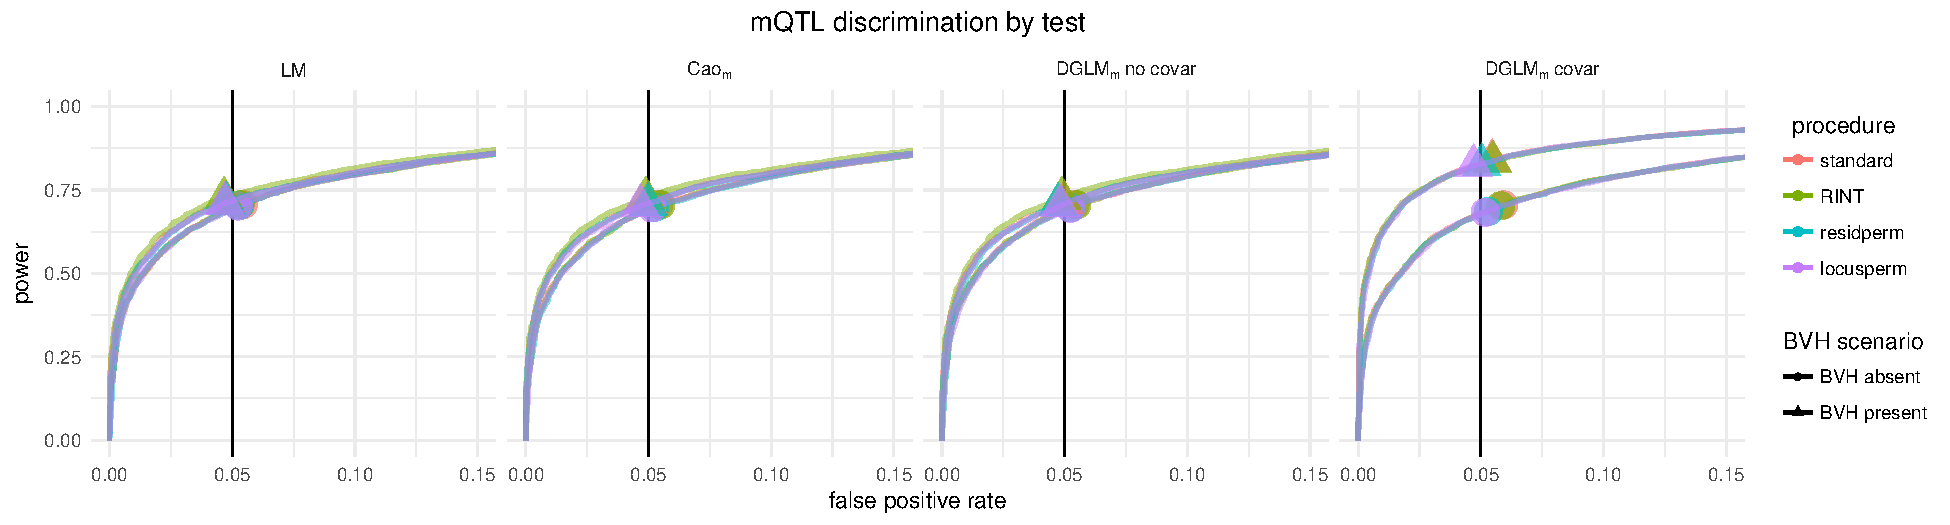
\includegraphics[height = 4.5cm]{images/rocs_mqtl_all_facet_by_test.pdf}
          \caption{
          All test-evaluations accurately control FPR. \DGLMm with BVH of known source is the most powerful test.}
      \vspace*{1cm}
      \end{subfigure}
      \begin{subfigure}{\textwidth}
          \centering
          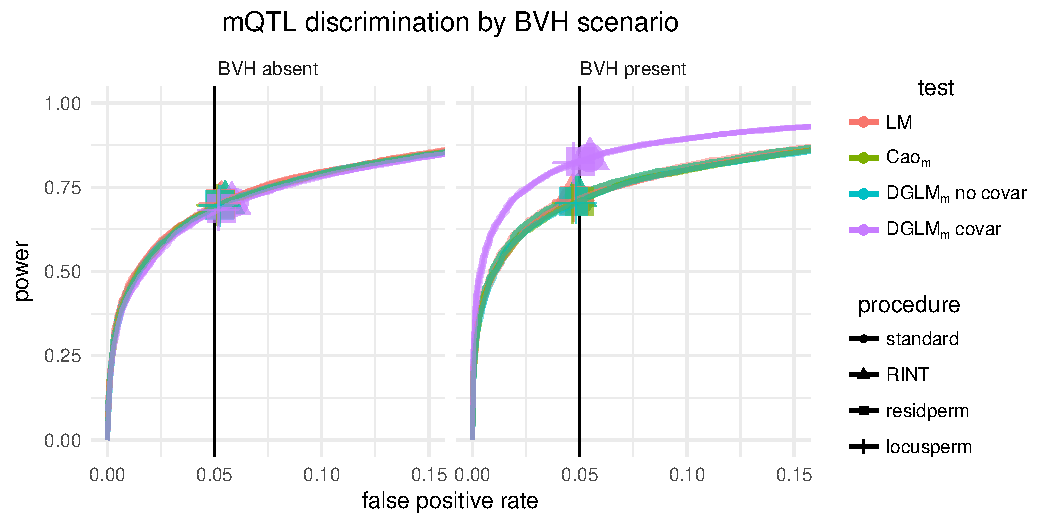
\includegraphics[height = 4.5cm]{images/rocs_mqtl_all_facet_by_bvh.pdf}
          \caption{
          Within BVH scenarios, all mQTL tests perform equivalently.}
      \vspace*{1cm}
      \end{subfigure}
      \begin{subfigure}{\textwidth}
          \centering
          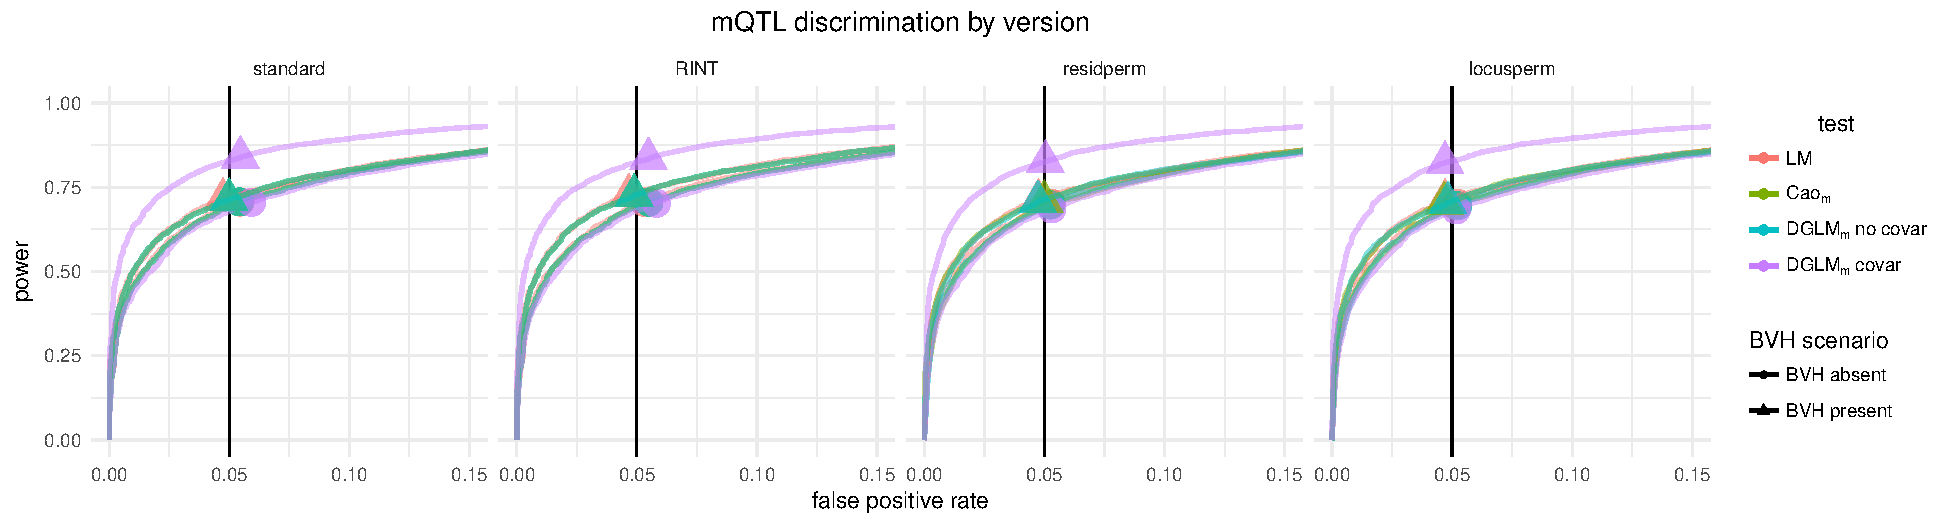
\includegraphics[height = 4.5cm]{images/rocs_mqtl_all_facet_by_eval.pdf}
          \caption{
          \DGLMm outperforms all other tests across all evaluation methods.}
      \end{subfigure}
      \caption[
        ROC Curves for mQTL tests in the detection of mQTL.
      ]
      {
        ROC Curves for mQTL tests in the detection of mQTL.
        The same 32 ROC curves are plotted three times, organized by (a) test, (b) BVH scenario, and (c) version to allow for comparisons across all dimensions.
      }
      \label{fig:mqtl_rocs_supp}
  \end{figure}


  \begin{figure}[ht]
      \begin{subfigure}{\textwidth}
          \centering
          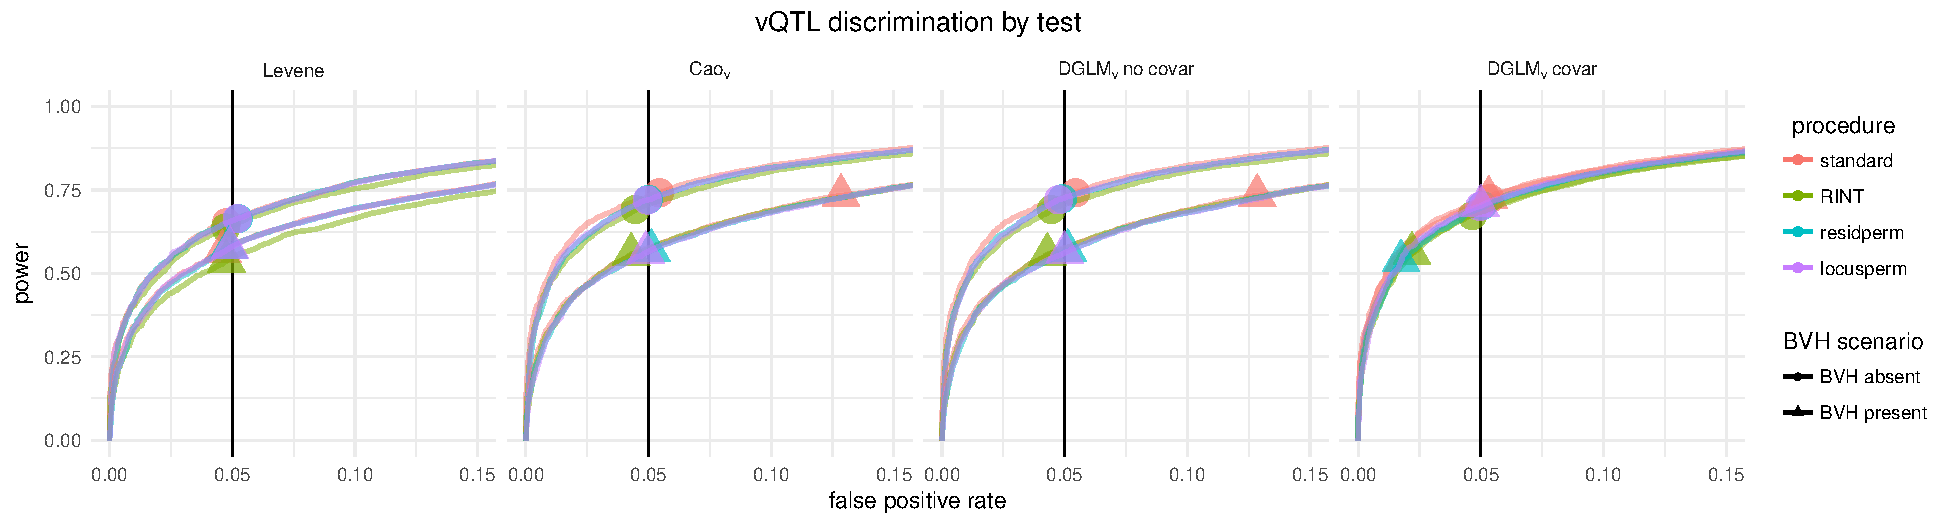
\includegraphics[height = 4.5cm]{images/rocs_vqtl_all_facet_by_test.pdf}
          \caption{
          Levene's test accurately conrols FPR in all scenarios.\Caov and \DGLMv have inflated FPR in the presence of BVH of uknnown source.
          \DGLMv's RINT and residperm versions are anti-conservative in the presence of BVH of known source.}
      \vspace*{1cm}
      \end{subfigure}
      \begin{subfigure}{\textwidth}
          \centering
          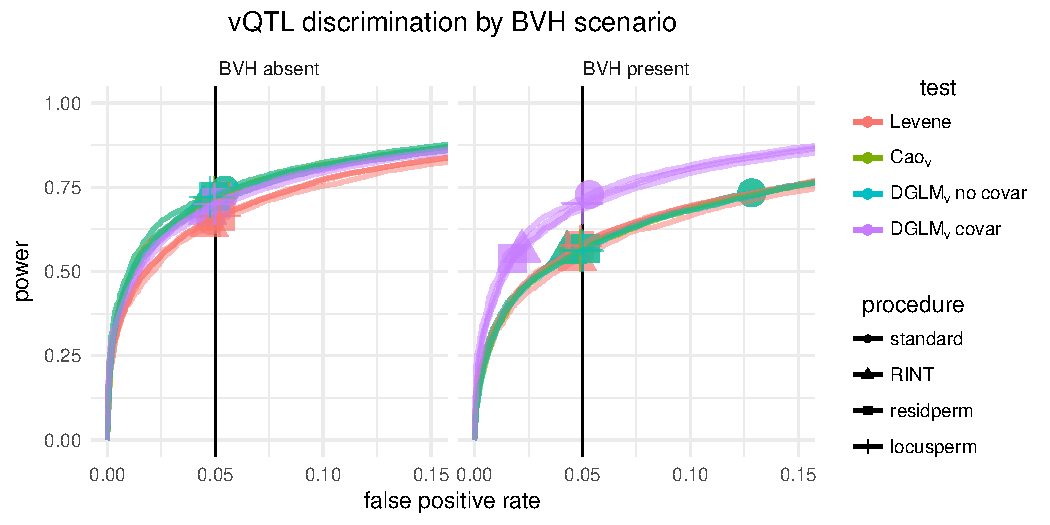
\includegraphics[height = 4.5cm]{images/rocs_vqtl_all_facet_by_bvh.pdf}
          \caption{
          In the absence of BVH, \Lev is less powerful than \Caov and \DGLMv.
          In the face of BVH of uknown source, all tests suffer decreased power, except \DGLMv's standard version, which fails to accurately control FPR.
          In the scenario with BVH of known source, \DGLMv recovers most of the power lost with introduction of BVH, but its RINT and residperm versions are anti-conservative.
          }
      \vspace*{1cm}
      \end{subfigure}
      \begin{subfigure}{\textwidth}
          \centering
          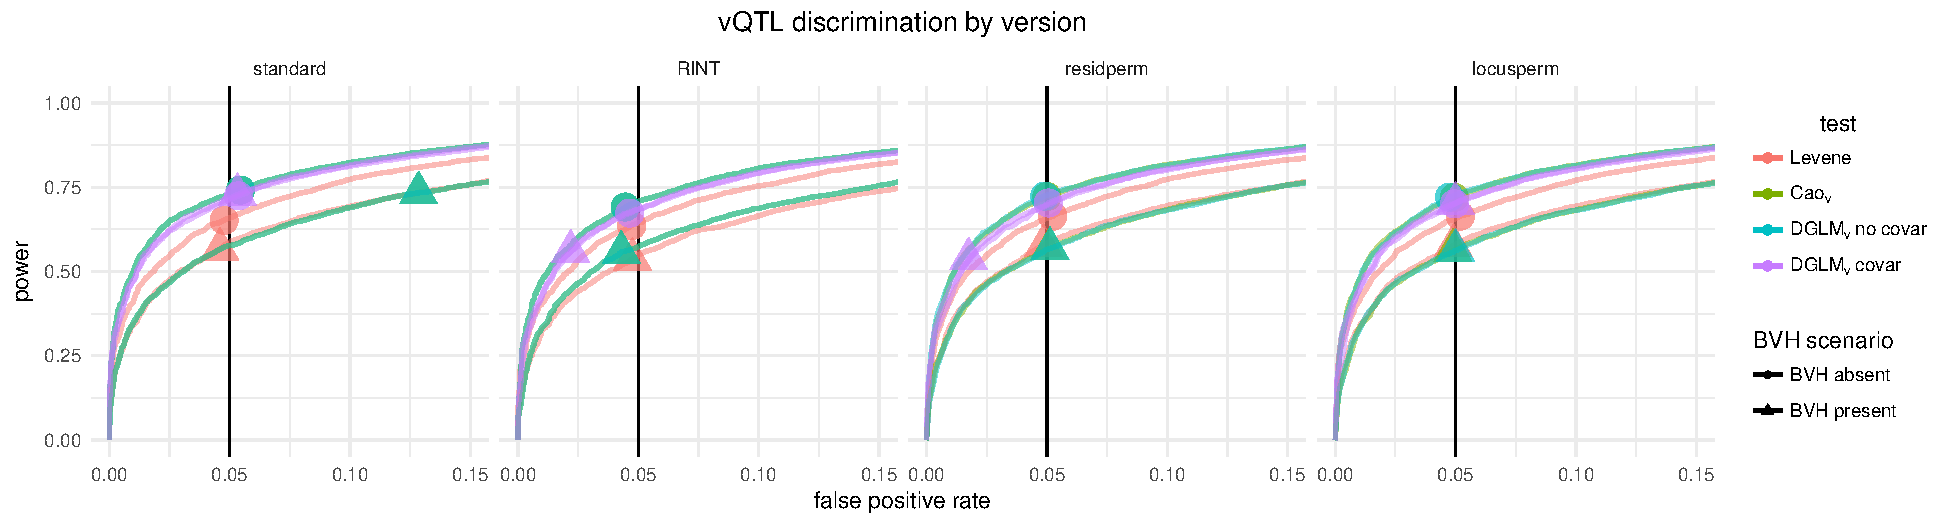
\includegraphics[height = 4.5cm]{images/rocs_vqtl_all_facet_by_eval.pdf}
          \caption{
          The only version of \DGLMv that accurately controls FPR across all BVH scenarios is locusperm.
          Its standard version is anticonservative in the presence of BVH of unknown source and its RINT and residperm versions are conservative in the presence of BVH of known source.
          }
      \end{subfigure}
      \caption[
        ROC Curves for vQTL tests in the detection of vQTL.
      ]
      {
        ROC Curves for vQTL tests in the detection of vQTL.
        The same 32 ROC curves are plotted three times, organized by (a) test, (b) BVH scenario, and (c) version to allow for comparisons across all dimensions.
      }
      \label{fig:vqtl_rocs_supp}
  \end{figure}


  \begin{figure}[ht]
      \begin{subfigure}{\textwidth}
          \centering
          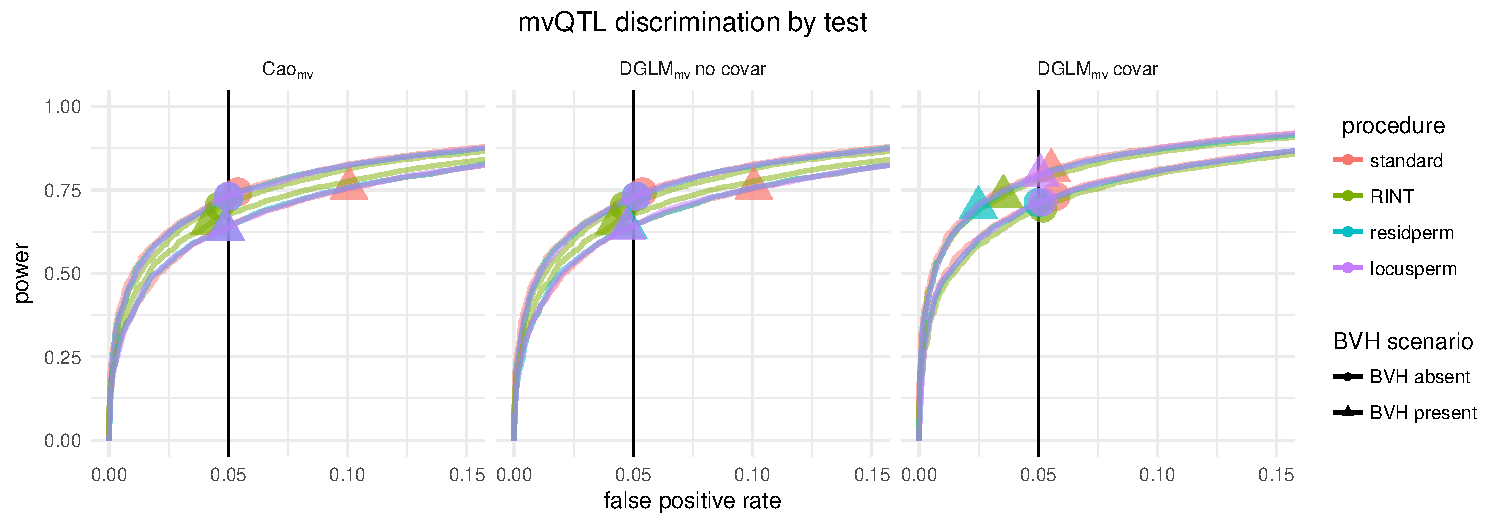
\includegraphics[height = 4.5cm]{images/rocs_mvqtl_all_facet_by_test.pdf}
          \caption{
          \Caomv and \DGLMmv both suffer a decrease in discrimiation (down and right shift of ROC curve) in the presence of BVH of unknown (or unmodeled) source.
          Only \DGLMmv can accommodate the source when it is known and therefore can achieve superior discrimination in that case.
          The standard and locusperm versions of \DGLMmv accurately control FPR.
          }
      \vspace*{0.5cm}
      \end{subfigure}
      \begin{subfigure}{\textwidth}
          \centering
          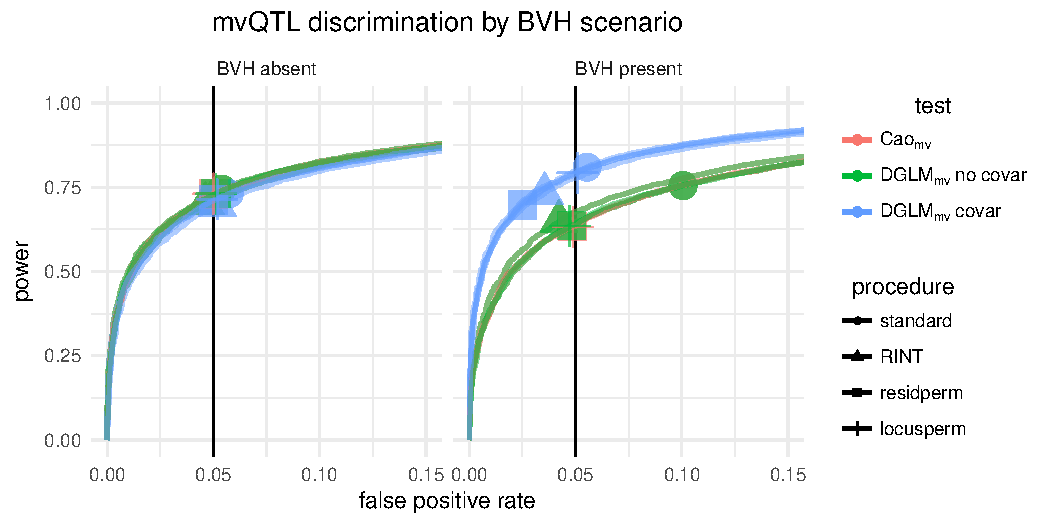
\includegraphics[height = 4.5cm]{images/rocs_mvqtl_all_facet_by_bvh.pdf}
          \caption{
          In the absence of BVH, both mvQTL tests accurately control FPR and have similar power.
          In the presence of BVH of uknown source, the standard version of both mvQTL tests is anti-conservative and the other three versions maintain FPR control but suffer a decrease in power compared to the no-BVH scenario.
          Only \DGLMmv can incorporate information on the BVH-driving covariate.
          It achieves increased power and accurately controls FPR in its standard and locusperm versions and is conservative in its RINT and locusperm versions.
          }
      \vspace*{0.5cm}
      \end{subfigure}
      \begin{subfigure}{\textwidth}
          \centering
          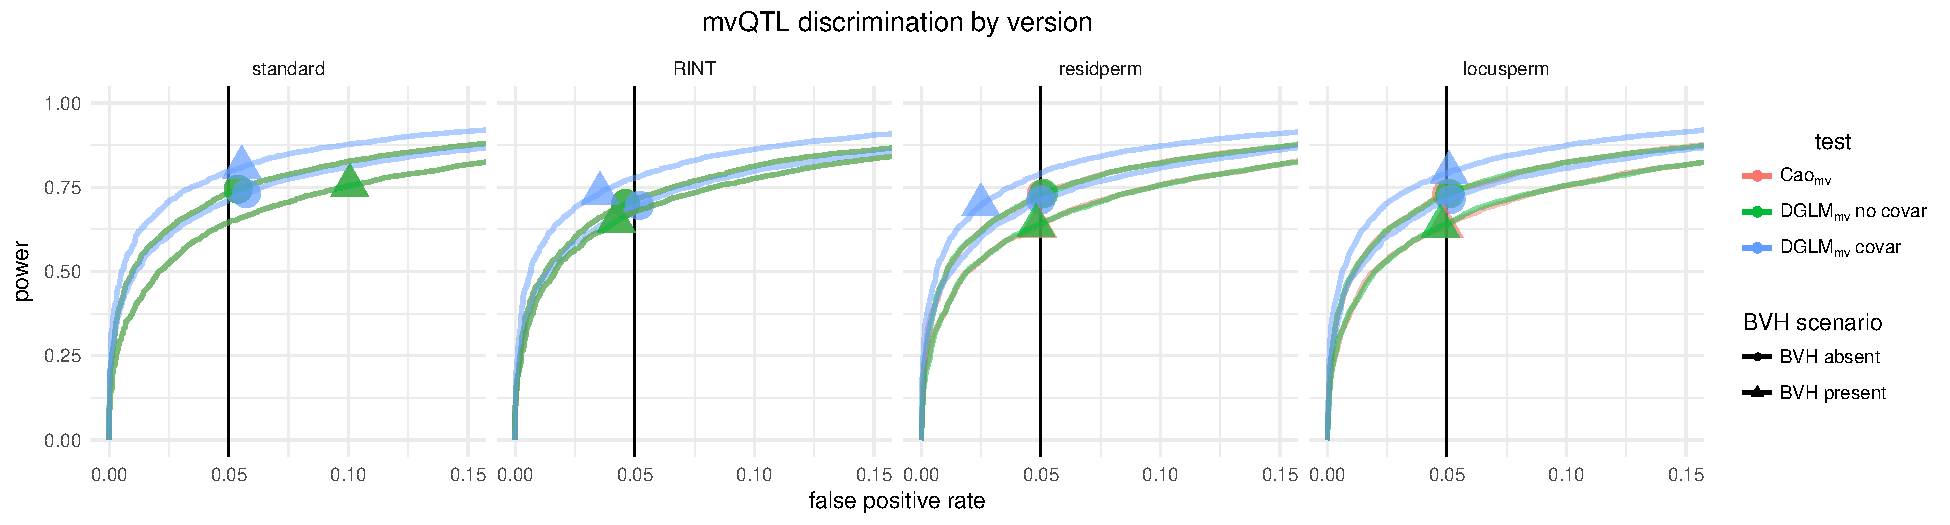
\includegraphics[height = 4.5cm]{images/rocs_mvqtl_all_facet_by_eval.pdf}
          \caption{
          Only the locusperm version accurately controls FPR in all scenarios.
          The standard version of both tests are anti-conservative in the presence of BVH of known source and the RINT and residperm versions are conservative in \DGLMmv the presence of BVH of known source.
          }
      \end{subfigure}
      \caption[
        ROC Curves for mvQTL tests in the detection of mvQTL.
      ]
      {
        ROC Curves for mvQTL tests in the detection of mvQTL.
        The same 24 ROC curves are plotted three times, organized by (a) test, (b) BVH scenario, and (c) version to allow for comparisons across all dimensions.
      }
      \label{fig:mvqtl_rocs_supp}
  \end{figure}

\FloatBarrier
\clearpage
\subsection{QQ Plots}
  \begin{figure}[h!]
      \centering
      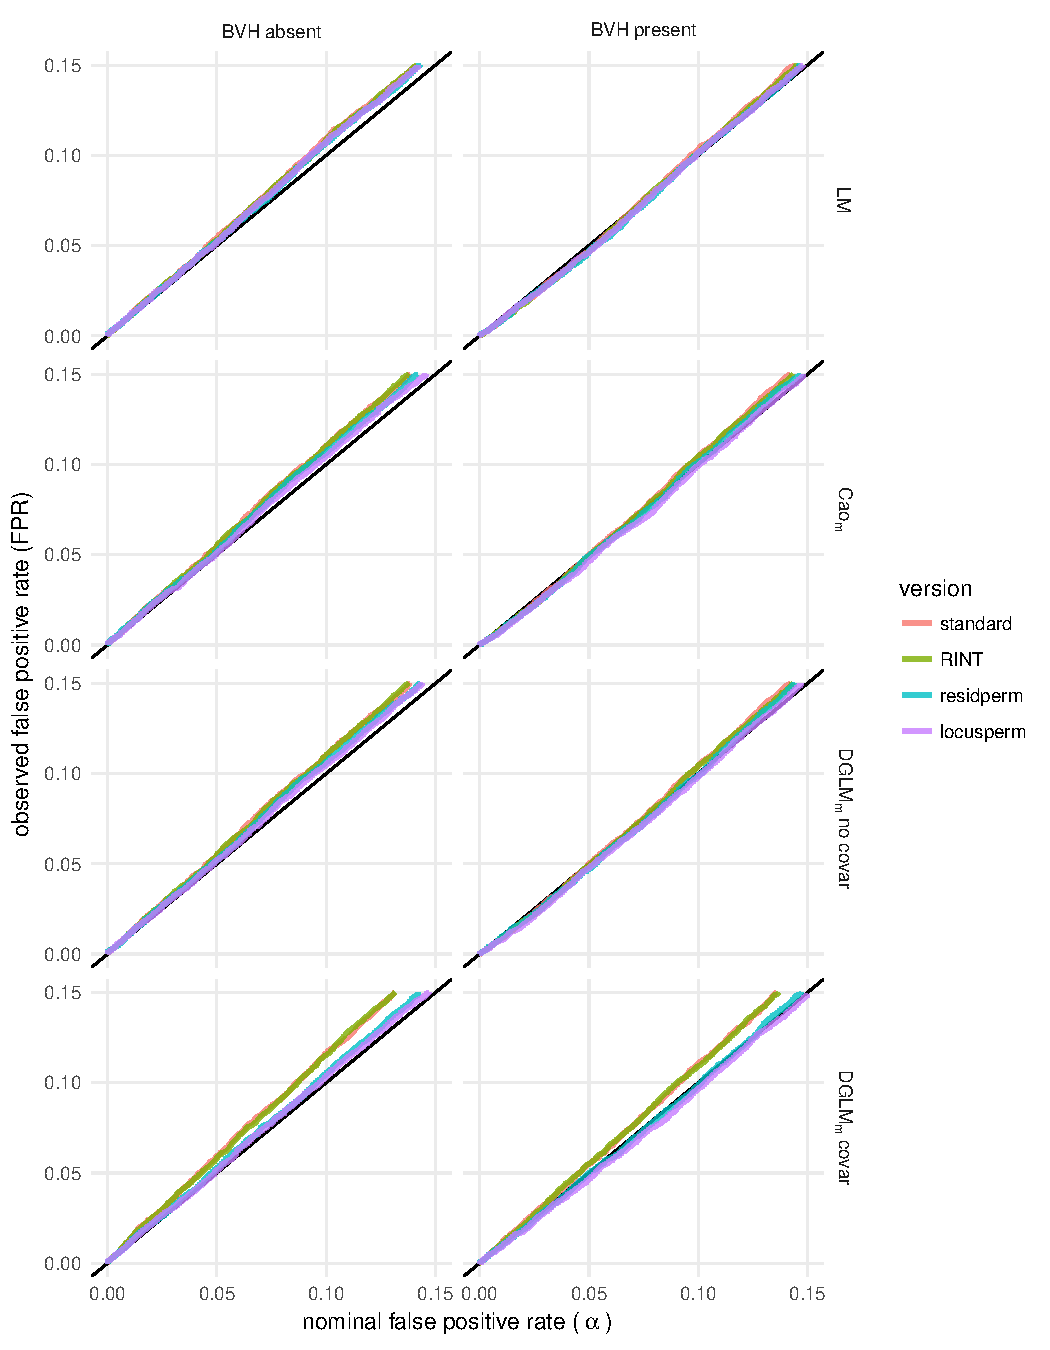
\includegraphics[width = 0.9\linewidth]{images/mqtl_null_qqs.pdf}
      \caption[
        The empirical false positive rate of each mQTL test-version for each nominal false positive rate, $\alpha$, in {[}0, 0.1{]}.
      ]
      {
        The empirical false positive rate of each mQTL test-version for each nominal false positive rate, $\alpha$, in {[}0, 0.1{]}.
        A test that accurately controls FPR will have $\text{empirical FPR}=\alpha$ for all value of $\alpha$.
        All mQTL tests accurately control FPR.
      }
      \label{fig:mqtl_tests_null_qqs}
  \end{figure}

  \begin{figure}[hp]
      \centering
      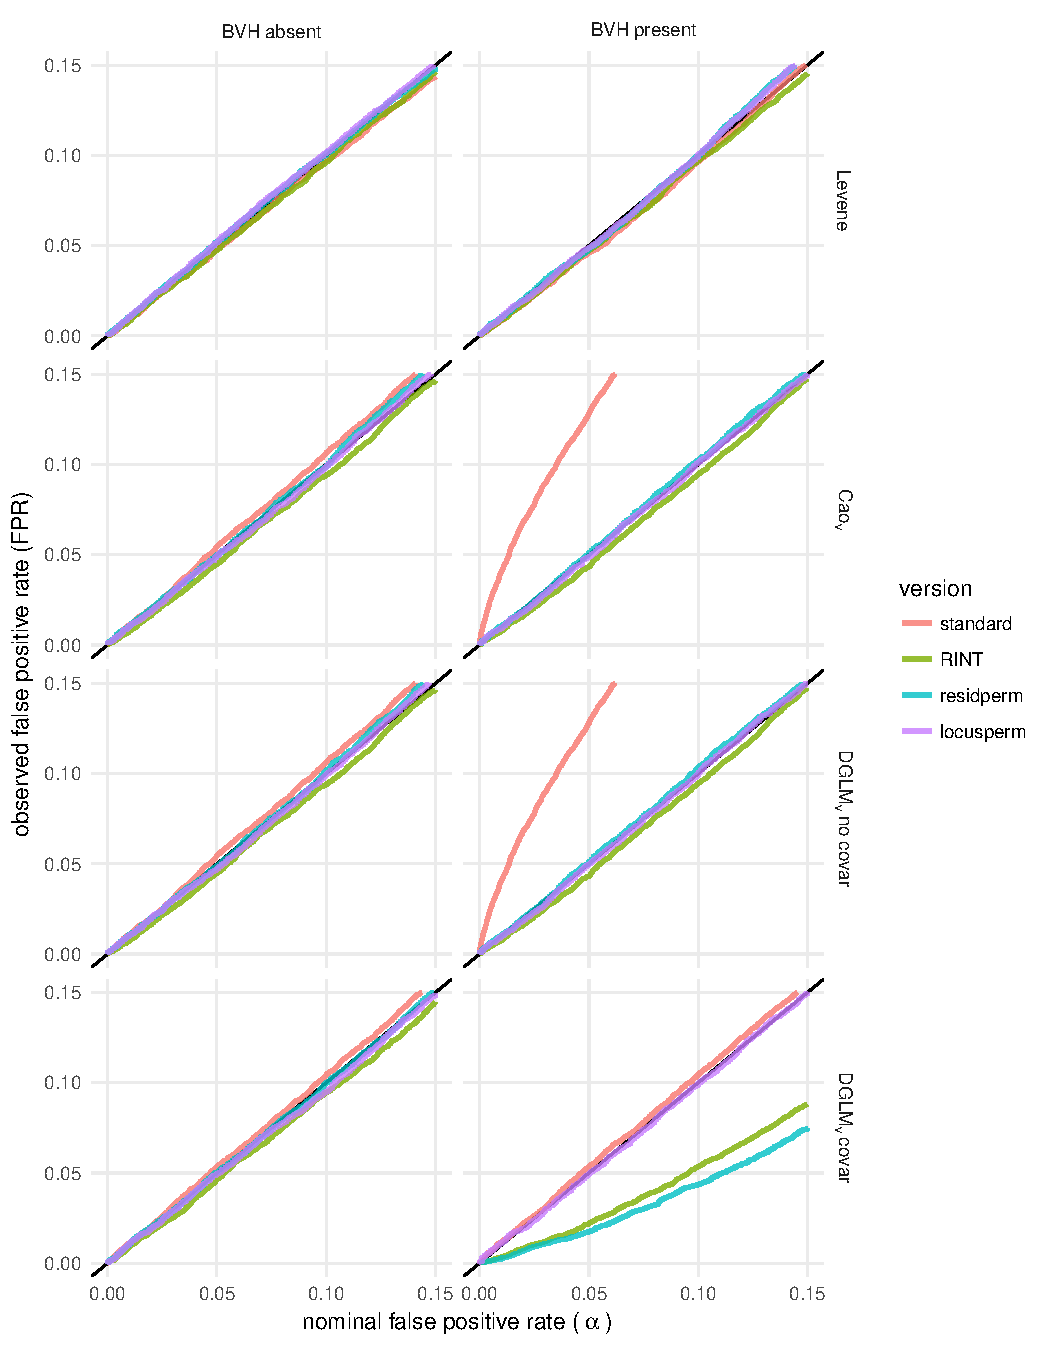
\includegraphics[width = \linewidth]{images/vqtl_null_qqs.pdf}
      \caption[
        The empirical false positive rate of each vQTL test-version for each nominal false positive rate, $\alpha$, in {[}0, 0.1{]}.
      ]
      {
        The empirical false positive rate of each vQTL test-version for each nominal false positive rate, $\alpha$, in {[}0, 0.1{]}.
        A test that accurately controls FPR will have $\text{empirical FPR}=\alpha$ for all value of $\alpha$.
        Amongst vQTL tests, \Caov has conservative behavior in the presence of BVH when the standard procedure is used, and \DGLMv has anti-conservative behavior when the RINT and residperm procedures are used.
      }
      \label{fig:vqtl_tests_null_qqs}
  \end{figure}

  \begin{figure}[hp]
      \centering
      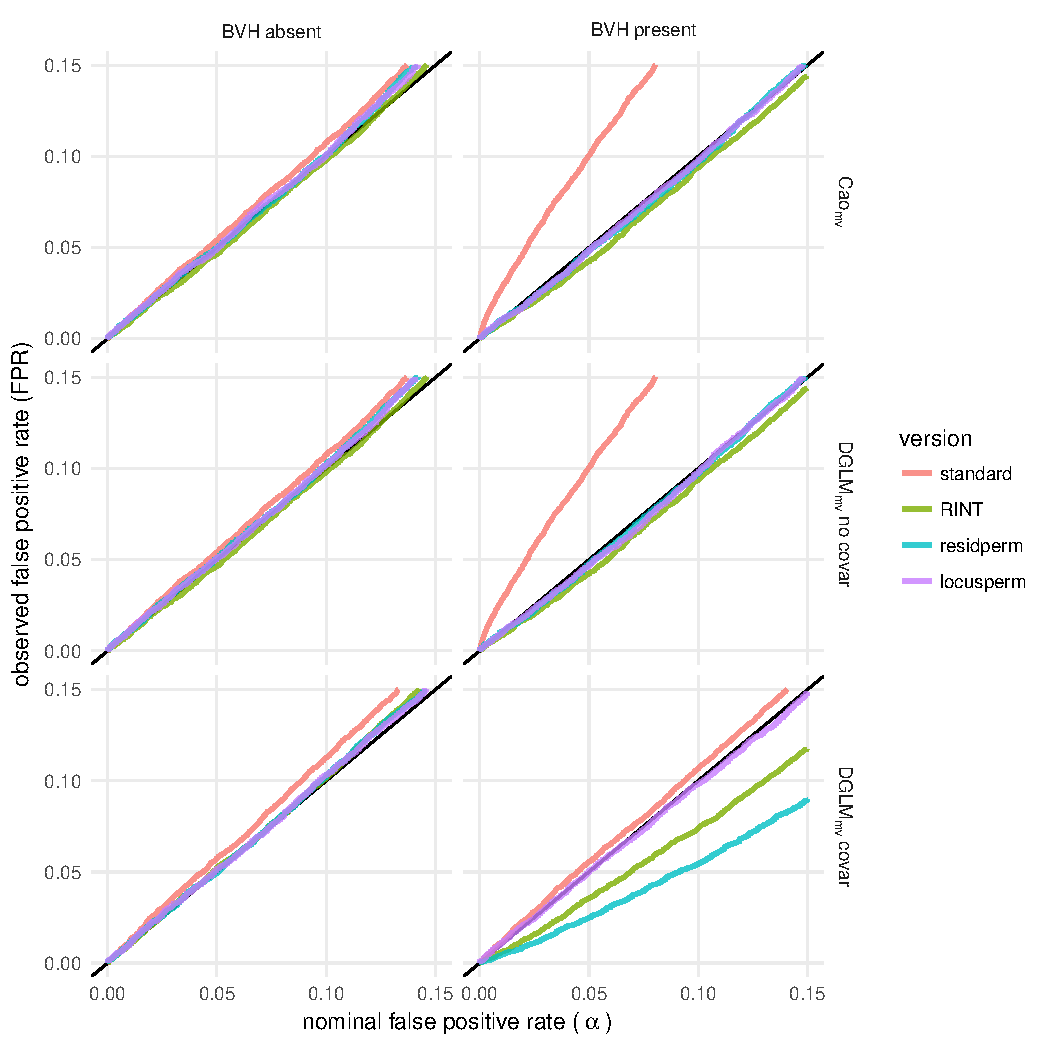
\includegraphics[height = 5in]{images/mvqtl_null_qqs.pdf}
      \caption[
        The empirical false positive rate of each mvQTL test-version for each nominal false positive rate, $\alpha$, in {[}0, 0.1{]}.
      ]
      {
        The empirical false positive rate of each mvQTL test-version for each nominal false positive rate, $\alpha$, in {[}0, 0.1{]}.
        A test that accurately controls FPR will have $\text{empirical FPR}=\alpha$ for all value of $\alpha$.
        mvQTL tests show the same pattern of deviation from accurate FPR control as vQTL tests (\autoref{fig:vqtl_tests_null_qqs}), but to a lesser extent.
      }
      \label{fig:mvqtl_tests_null_qqs}
  \end{figure}

\FloatBarrier
\clearpage
\subsection{False Positive Rates of mQTL tests}

  \renewcommand{\arraystretch}{1.0}

  \begin{table}[ht]
      \centering
      \begin{tabular}{p{2cm}ll llll lll}
      \cmidrule[1pt]{1-10}
         &  & \multicolumn{4}{c}{BVH absent} & \multicolumn{4}{c}{BVH present}\\
         \cmidrule(lr){3-6} \cmidrule(lr){7-10} 
         test & version & null & mQTL & vQTL & mvQTL & null & mQTL & vQTL & mvQTL\\
          \cmidrule[1pt]{1-10}
          LM & standard & 0.054 & 0.706 & 0.055 & 0.504 & 0.047 & 0.713 & 0.051 & 0.510 \\ 
           & RINT & 0.053 & 0.706 & 0.053 & 0.490 & 0.047 & 0.727 & 0.047 & 0.522 \\ 
           & residperm & 0.052 & 0.700 & 0.053 & 0.495 & 0.046 & 0.708 & 0.050 & 0.506 \\ 
           & locusperm & 0.051 & 0.698 & 0.054 & 0.494 & 0.046 & 0.708 & 0.050 & 0.506 \\ 
          \cmidrule[0.1pt]{1-10}
          \Caom & standard & 0.055 & 0.707 & 0.049 & 0.511 & 0.050 & 0.713 & 0.048 & 0.522 \\ 
           & RINT & 0.055 & 0.706 & 0.047 & 0.501 & 0.049 & 0.726 & 0.047 & 0.534 \\ 
           & residperm & 0.051 & 0.696 & 0.046 & 0.504 & 0.049 & 0.704 & 0.046 & 0.512 \\ 
           & locusperm & 0.050 & 0.693 & 0.046 & 0.499 & 0.046 & 0.699 & 0.045 & 0.510 \\ 
          \cmidrule[0.1pt]{1-10}
          \multirow{2}{2cm}{\DGLMm\newline no~covar} & standard & 0.055 & 0.707 & 0.049 & 0.511 & 0.050 & 0.713 & 0.048 & 0.522 \\ 
           & RINT & 0.055 & 0.706 & 0.047 & 0.501 & 0.049 & 0.726 & 0.047 & 0.534 \\ 
           & residperm & 0.052 & 0.695 & 0.046 & 0.502 & 0.047 & 0.703 & 0.048 & 0.513 \\ 
           & locusperm & 0.051 & 0.693 & 0.044 & 0.500 & 0.047 & 0.700 & 0.044 & 0.509 \\ 
          \cmidrule[0.1pt]{1-10}
          \multirow{2}{2cm}{\DGLMm\newline with~covar} & standard & 0.059 & 0.705 & 0.052 & 0.512 & 0.055 & 0.838 & 0.057 & 0.658 \\ 
           & RINT & 0.058 & 0.703 & 0.050 & 0.503 & 0.055 & 0.835 & 0.056 & 0.651 \\ 
           & residperm & 0.052 & 0.683 & 0.044 & 0.490 & 0.049 & 0.823 & 0.051 & 0.634 \\ 
           & locusperm & 0.051 & 0.680 & 0.045 & 0.485 & 0.046 & 0.821 & 0.049 & 0.630 \\ 
        \hline
      \end{tabular}
      \caption[
        Positive rates of mQTL tests in extended scenarios.
      ]
      {
        Positive rates of all four mQTL tests in all scenarios based on 10,000 simulations, 1,000 permutations each to estimate empirical null distributions (residperm and locusperm), and a cutoff of $p = 0.05$.
        Note that in all cases the DGLM test without the covariate had identical or very nearly identical FPR to the Cao test that tests for the same kind of QTL.
      }
      \label{tab:mqtl_fpr}
  \end{table}


\FloatBarrier
\clearpage
\subsection{False Positive Rates of vQTL tests}

  \renewcommand{\arraystretch}{1.0}

  \begin{table}[ht]
      \centering
      \begin{tabular}{lll llll lll}
      \cmidrule[1pt]{1-10}
         &  & \multicolumn{4}{c}{BVH absent} & \multicolumn{4}{c}{BVH present}\\
         \cmidrule(lr){3-6} \cmidrule(lr){7-10} 
         test & version & null & mQTL & vQTL & mvQTL & null & mQTL & vQTL & mvQTL\\
          \cmidrule[1pt]{1-10}
          \Lev & standard & 0.048 & 0.045 & 0.653 & 0.466 & 0.046 & 0.048 & 0.566 & 0.387 \\ 
           & RINT & 0.048 & 0.040 & 0.637 & 0.422 & 0.047 & 0.043 & 0.536 & 0.339 \\ 
           & residperm & 0.052 & 0.049 & 0.661 & 0.477 & 0.048 & 0.051 & 0.573 & 0.394 \\ 
           & locusperm & 0.051 & 0.050 & 0.661 & 0.475 & 0.048 & 0.050 & 0.573 & 0.393 \\ 
          \cmidrule[0.1pt]{1-10}
          \Caov & standard & 0.054 & 0.051 & 0.742 & 0.543 & 0.128 & 0.124 & 0.733 & 0.571 \\ 
           & RINT & 0.045 & 0.040 & 0.691 & 0.468 & 0.043 & 0.047 & 0.557 & 0.365 \\ 
           & residperm & 0.049 & 0.048 & 0.720 & 0.520 & 0.050 & 0.050 & 0.565 & 0.388 \\ 
           & locusperm & 0.048 & 0.048 & 0.718 & 0.517 & 0.048 & 0.048 & 0.559 & 0.382 \\ 
          \cmidrule[0.1pt]{1-10}
          \DGLMv\newline no~covar & standard & 0.054 & 0.051 & 0.742 & 0.543 & 0.128 & 0.124 & 0.733 & 0.571 \\ 
           & RINT & 0.045 & 0.040 & 0.691 & 0.468 & 0.043 & 0.047 & 0.557 & 0.365 \\ 
           & residperm & 0.048 & 0.049 & 0.721 & 0.522 & 0.050 & 0.050 & 0.565 & 0.388 \\ 
           & locusperm & 0.047 & 0.048 & 0.718 & 0.519 & 0.049 & 0.049 & 0.559 & 0.381 \\ 
          \cmidrule[0.1pt]{1-10}
          \multirow{2}{2cm}{\DGLMv\newline with~covar} & standard & 0.053 & 0.053 & 0.724 & 0.525 & 0.054 & 0.054 & 0.729 & 0.531 \\ 
           & RINT & 0.046 & 0.041 & 0.673 & 0.453 & 0.022 & 0.022 & 0.560 & 0.341 \\ 
           & residperm & 0.050 & 0.047 & 0.699 & 0.501 & 0.017 & 0.015 & 0.533 & 0.325 \\ 
           & locusperm & 0.049 & 0.048 & 0.698 & 0.501 & 0.049 & 0.050 & 0.700 & 0.498 \\ 
        \hline
      \end{tabular}
      \caption[
        Positive rates of vQTL tests in extended scenarios.
      ]
      {
        Positive rates of all four vQTL tests in all scenarios based on 10,000 simulations, 1,000 permutations each to estimate empirical null distributions (residperm and locusperm), and a cutoff of $p = 0.05$.
        Note that in all cases the DGLM test without the covariate had identical or very nearly identical FPR to the Cao test that tests for the same kind of QTL.
      }
      \label{tab:vqtl_fpr}
  \end{table}



\FloatBarrier
\clearpage
\subsection{False Positive Rates of mvQTL tests}

  \renewcommand{\arraystretch}{1.0}

  \begin{table}[ht]
      \centering
      \begin{tabular}{p{2cm}ll llll lll}
      \cmidrule[1pt]{1-10}
         &  & \multicolumn{4}{c}{BVH absent} & \multicolumn{4}{c}{BVH present}\\
         \cmidrule(lr){3-6} \cmidrule(lr){7-10} 
         test & version & null & mQTL & vQTL & mvQTL & null & mQTL & vQTL & mvQTL\\
          \cmidrule[1pt]{1-10}
          \Caomv & standard & 0.054 & 0.594 & 0.637 & 0.745 & 0.100 & 0.651 & 0.644 & 0.755 \\ 
           & RINT & 0.046 & 0.585 & 0.570 & 0.703 & 0.042 & 0.608 & 0.435 & 0.649 \\ 
           & residperm & 0.049 & 0.587 & 0.609 & 0.726 & 0.048 & 0.523 & 0.505 & 0.628 \\ 
           & locusperm & 0.049 & 0.588 & 0.611 & 0.728 & 0.047 & 0.523 & 0.504 & 0.630 \\ 
          \cmidrule[0.1pt]{1-10}
          \multirow{2}{2cm}{\DGLMmv\newline no~covar} & standard & 0.054 & 0.594 & 0.637 & 0.745 & 0.100 & 0.651 & 0.644 & 0.755 \\ 
           & RINT & 0.046 & 0.585 & 0.570 & 0.703 & 0.042 & 0.608 & 0.435 & 0.649 \\ 
           & residperm & 0.050 & 0.588 & 0.610 & 0.728 & 0.047 & 0.524 & 0.503 & 0.632 \\ 
           & locusperm & 0.050 & 0.587 & 0.612 & 0.728 & 0.046 & 0.522 & 0.505 & 0.631 \\ 
          \cmidrule[0.1pt]{1-10}
          \multirow{2}{2cm}{\DGLMmv\newline with~covar} & standard & 0.058 & 0.596 & 0.620 & 0.732 & 0.055 & 0.745 & 0.621 & 0.809 \\ 
           & RINT & 0.052 & 0.587 & 0.554 & 0.696 & 0.036 & 0.720 & 0.432 & 0.732 \\ 
           & residperm & 0.049 & 0.576 & 0.582 & 0.710 & 0.025 & 0.625 & 0.457 & 0.694 \\ 
           & locusperm & 0.051 & 0.577 & 0.582 & 0.712 & 0.049 & 0.731 & 0.591 & 0.790 \\ 
        \hline
      \end{tabular}
      \caption[
        Positive rates of mvQTL tests in extended scenarios.
      ]
      {
        Positive rates of all three tests in all scenarios based on 10,000 simulations, 1,000 permutations each to estimate empirical null distributions (residperm and locusperm), and a cutoff of $p = 0.05$.
        Note that in all cases the DGLM test without the covariate had identical or very nearly identical FPR to the Cao test that tests for the same kind of QTL.
      }
      \label{tab:mvqtl_fpr}
  \end{table}

\FloatBarrier
\clearpage
\subsection{Cao's Profile-Likelihood Approximation is Extremely Accurate}
  \begin{figure}[h!]
    \begin{subfigure}{\linewidth}
        \caption{null simulations}
        \centering
        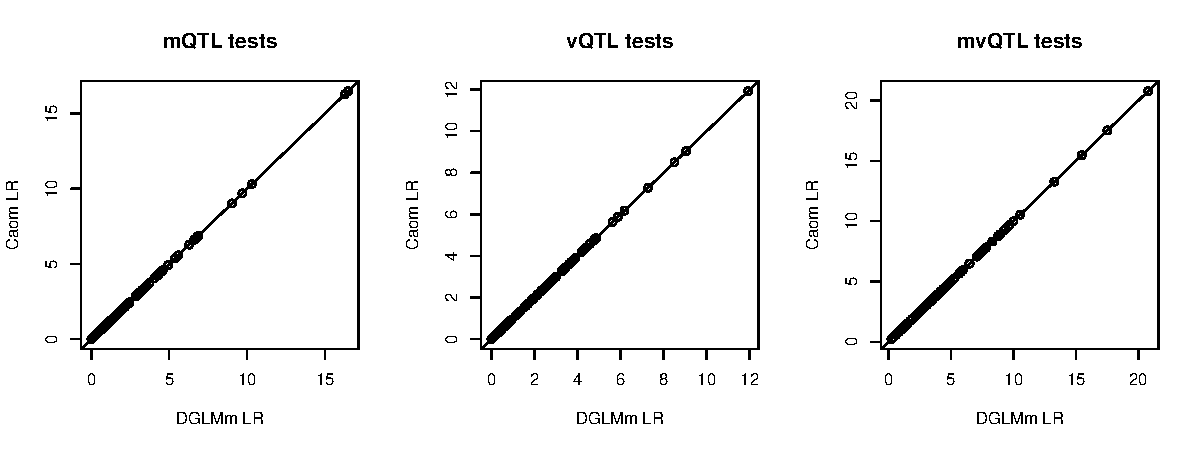
\includegraphics[width = 0.7\linewidth]{images/Cao_and_DGLM_indistinguishable_null.pdf}
    \end{subfigure}
     \begin{subfigure}{\linewidth}
        \caption{mQTL simulations}
        \centering
        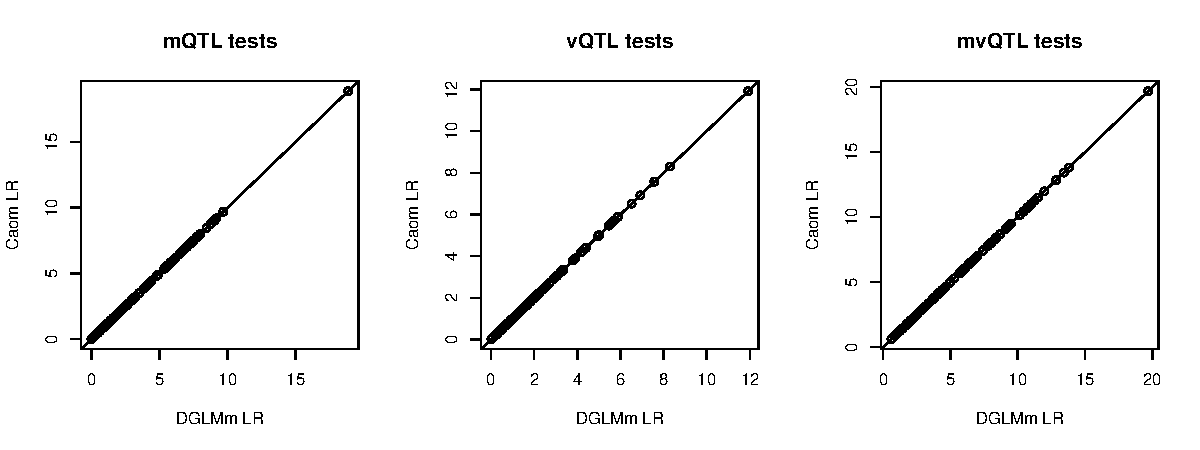
\includegraphics[width = 0.7\linewidth]{images/Cao_and_DGLM_indistinguishable_mqtl.pdf}
    \end{subfigure}
    \begin{subfigure}{\linewidth}
        \caption{vQTL simulations}
        \centering
        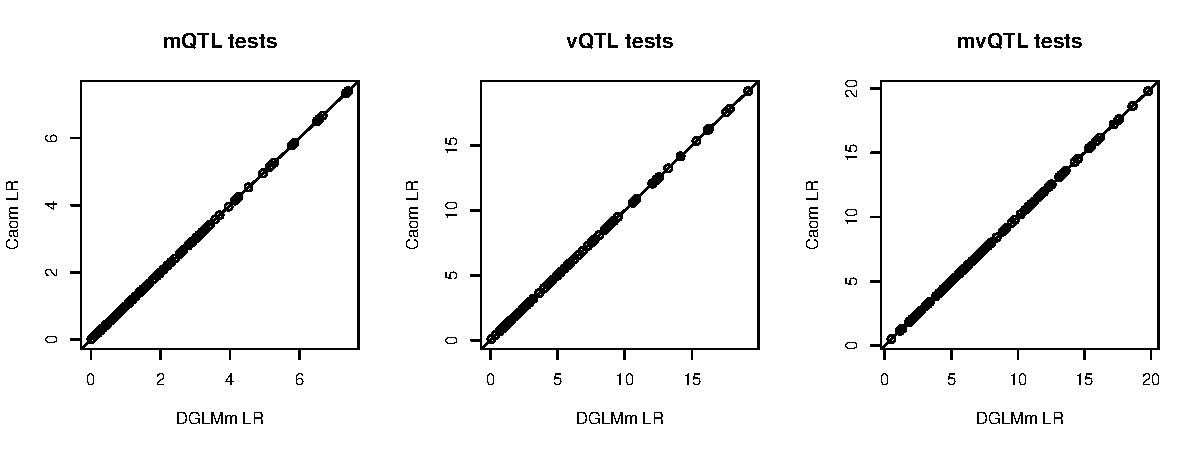
\includegraphics[width = 0.7\linewidth]{images/Cao_and_DGLM_indistinguishable_vqtl.pdf}
    \end{subfigure}
    \begin{subfigure}{\linewidth}
        \caption{mvQTL simulations}
        \centering
        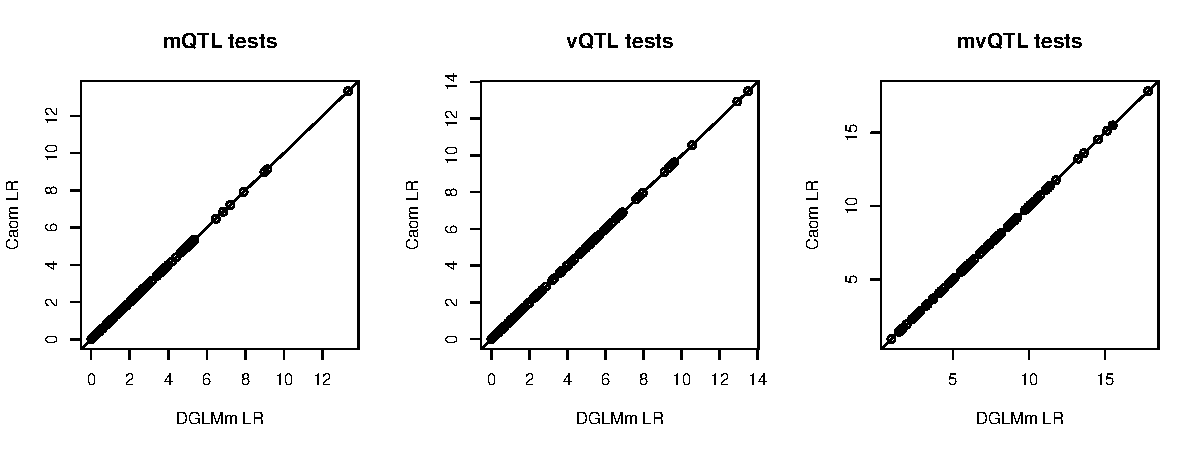
\includegraphics[width = 0.7\linewidth]{images/Cao_and_DGLM_indistinguishable_mvqtl.pdf}
    \end{subfigure}
    \caption{On simulated null loci, mQTL, vQTL, and mvQTL, Cao's profile likelihood method had identical likelihood ratio to DGLM when DGLM does not use any variance covariates.}
    \label{fig:cao_profile_accurate}
  \end{figure}


\FloatBarrier
\clearpage
\subsection{Cao's Tests for All Phenotypes with BVH}
  \begin{figure}[h]
    \begin{subfigure}{\linewidth}
      \centering
      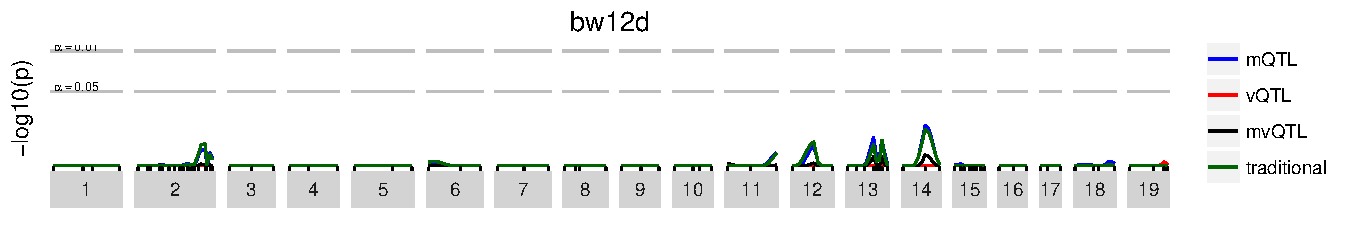
\includegraphics[width = 0.9\textwidth]{images/scan_cao_bw12d.pdf}
      \caption{Genome scan for bodyweight at twelve days}
      \label{fig:bw12d_cao_scan}
    \end{subfigure}
    \begin{subfigure}{\linewidth}
      \centering
      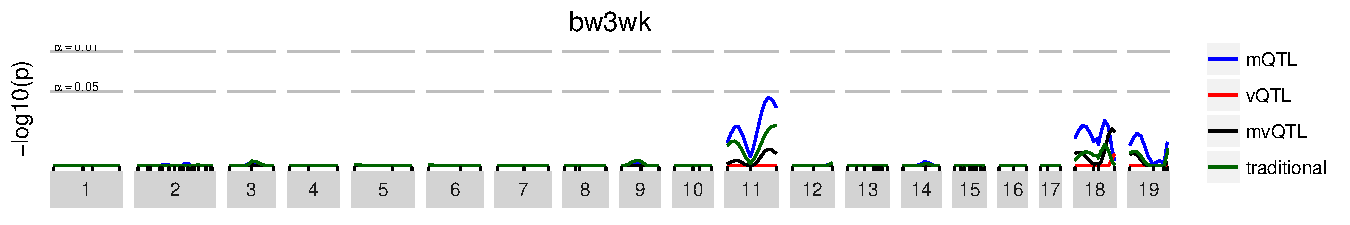
\includegraphics[width = 0.9\textwidth]{images/scan_cao_bw3wk.pdf}
      \caption{Genome scan for bodyweight at three weeks}
      \label{fig:bw3wk_cao_scan}
    \end{subfigure}
    \begin{subfigure}{\linewidth}
      \centering
      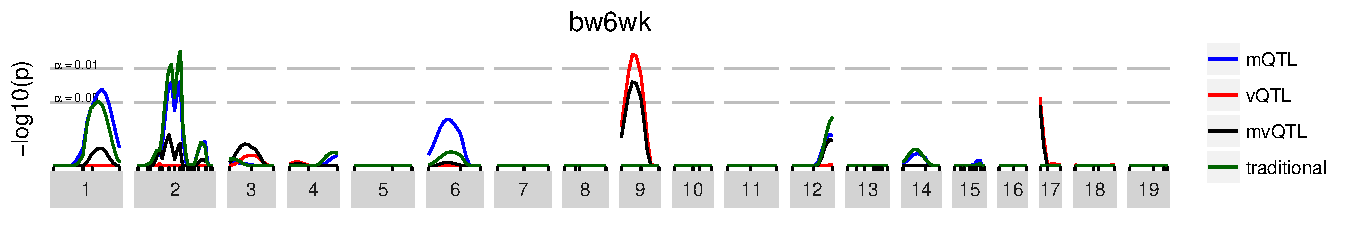
\includegraphics[width = 0.9\textwidth]{images/scan_cao_bw6wk.pdf}
      \caption{Genome scan for bodyweight at six weeks}
      \label{fig:bw6wk_cao_scan}
    \end{subfigure}
    \begin{subfigure}{\linewidth}
      \centering
      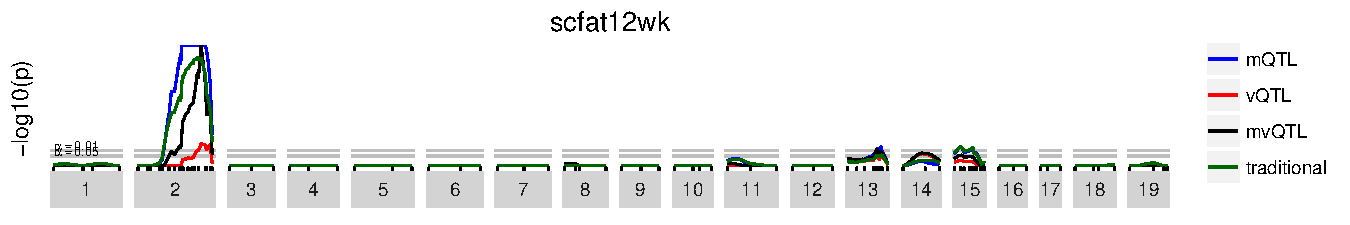
\includegraphics[width = 0.9\textwidth]{images/scan_cao_scfat12wk.pdf}
      \caption{Genome scan for subcutaneous fat pad thickness at twelve weeks}
      \label{fig:scfat12wk_cao_scan}
    \end{subfigure}
    \begin{subfigure}{\linewidth}
      \centering
      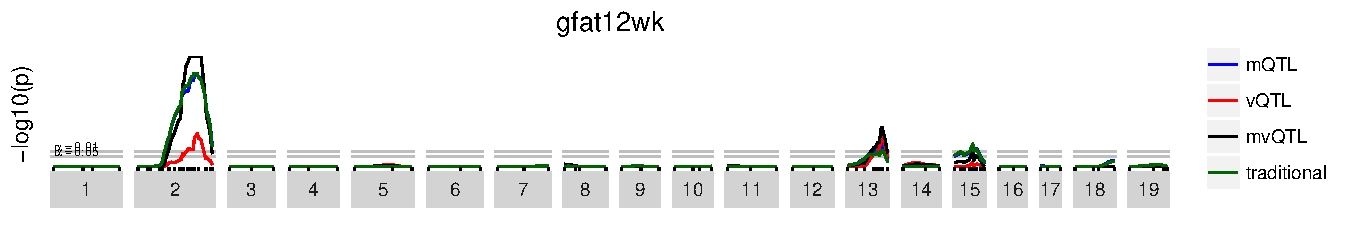
\includegraphics[width = 0.9\textwidth]{images/scan_cao_gfat12wk.pdf}
      \caption{Genome scan for gonadal fat pad thickness at twelve wees}
      \label{fig:gfat12wk_cao_scan}
    \end{subfigure}
    \caption{
      Genome scans conducted with the DGLM, without accounting for effects of sex and father on variance, shown by simulation to be identical to Cao's tests (\autoref{fig:cao_profile_accurate}, \autoref{tab:mqtl_fpr}, \autoref{tab:vqtl_fpr}, and \autoref{tab:mvqtl_fpr}).
    }
  \end{figure}
  

\FloatBarrier
\clearpage
\subsection{DGLM Tests for All Phenotypes with BVH}
  \begin{figure}[h]
    \begin{subfigure}{\linewidth}
      \centering
      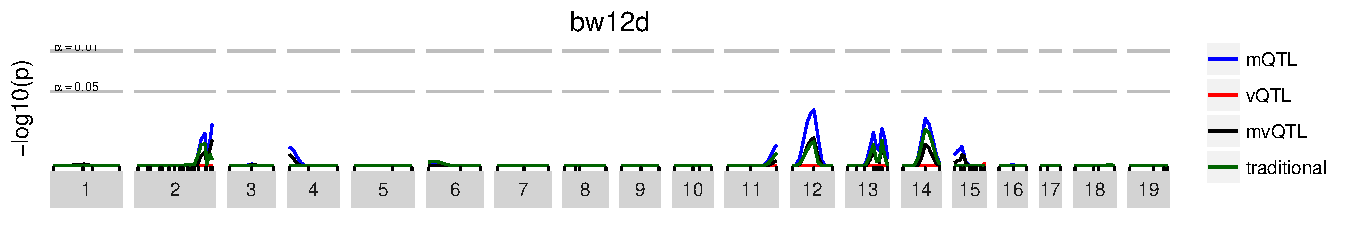
\includegraphics[width = 0.9\textwidth]{images/scan_dglm_bw12d.pdf}
      \caption{Genome scan for bodyweight at twelve days}
      \label{fig:bw12d_cao_scan}
    \end{subfigure}
    \begin{subfigure}{\linewidth}
      \centering
      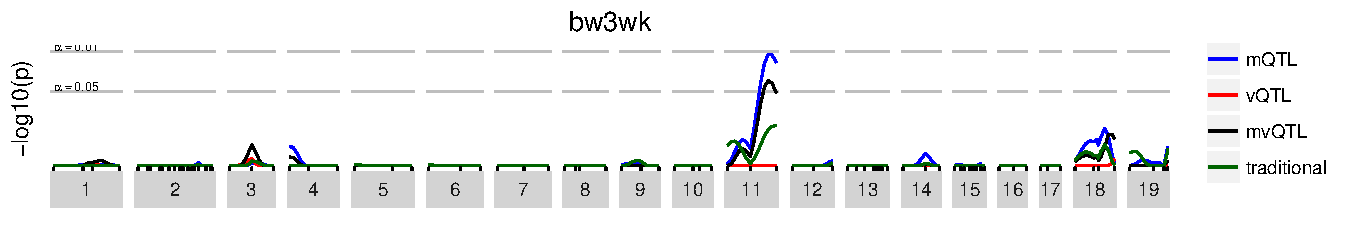
\includegraphics[width = 0.9\textwidth]{images/scan_dglm_bw3wk.pdf}
      \caption{Genome scan for bodyweight at three weeks}
      \label{fig:bw3wk_cao_scan}
    \end{subfigure}
    \begin{subfigure}{\linewidth}
      \centering
      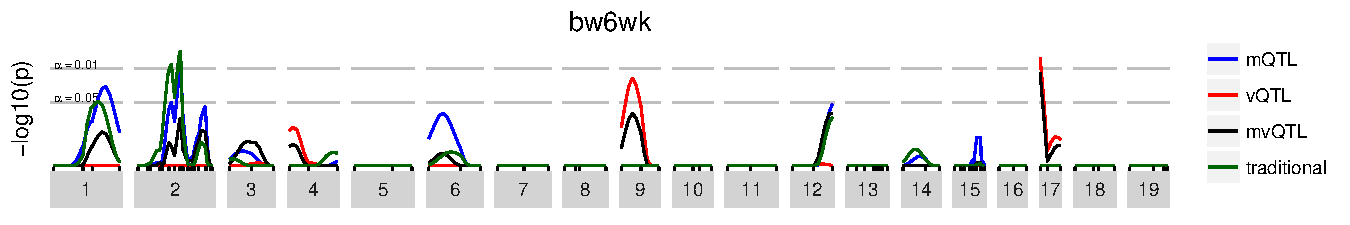
\includegraphics[width = 0.9\textwidth]{images/scan_dglm_bw6wk.pdf}
      \caption{Genome scan for bodyweight at six weeks}
      \label{fig:bw6wk_cao_scan}
    \end{subfigure}
    \begin{subfigure}{\linewidth}
      \centering
      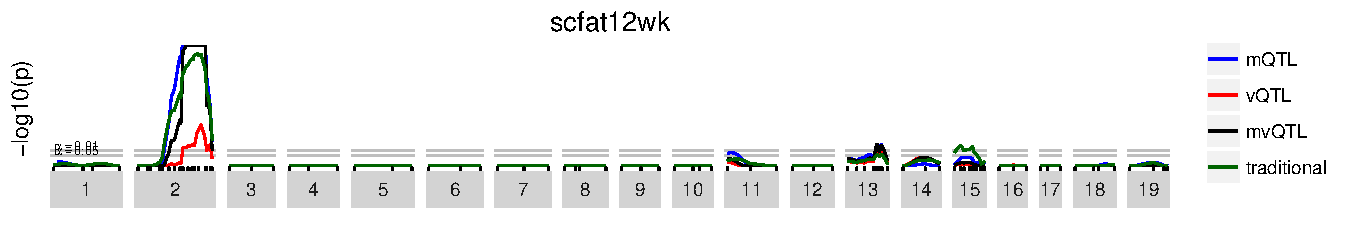
\includegraphics[width = 0.9\textwidth]{images/scan_dglm_scfat12wk.pdf}
      \caption{Genome scan for subcutaneous fat pad thickness at twelve weeks}
      \label{fig:scfat12wk_cao_scan}
    \end{subfigure}
    \begin{subfigure}{\linewidth}
      \centering
      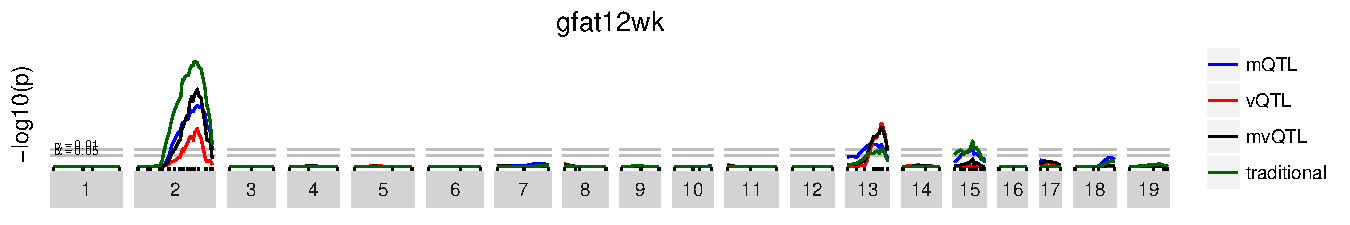
\includegraphics[width = 0.9\textwidth]{images/scan_dglm_gfat12wk.pdf}
      \caption{Genome scan for gonadal fat pad thickness at twelve wees}
      \label{fig:gfat12wk_cao_scan}
    \end{subfigure}
    \caption{
      Genome scans conducted with the DGLM, accounting for effects of sex and father on variance.
    }
  \end{figure}

